\documentclass[10pt,twocolumn,letterpaper]{article}

% សំភារៈផ្ទាល់ខ្លួនខ្ញុំ
\usepackage{booktabs}
% \usepackage{caption}
% \captionsetup[table]{skip=8pt}   % មានផលប៉ុណ្ណោះលើតារាង
\usepackage{stfloats}  % បន្ថែមបញ្ជូនទៅកានុប្បបញ្ជា
\usepackage{float}
% \usepackage[T1]{fontenc}

%–– ICU line-breaking for Khmer ––
\XeTeXlinebreaklocale "km"
\XeTeXlinebreakskip = 0pt plus 0pt minus 0pt
% \XeTeXlinebreakskip = 0pt plus 1pt

\usepackage{fontspec}

%–– define your two fonts ––
\newfontfamily\latinfont{Latin Modern Roman}        % for all Latin text
\newfontfamily\khmerfont[Script=Khmer]{Noto Sans Khmer} % for all Khmer text

%–– load ucharclasses to auto‐detect Unicode blocks ––
\usepackage{ucharclasses}

% default (everything outside Khmer) → Latin font
\setDefaultTransitions{\latinfont}{}

% when entering the Khmer Unicode block → switch to Khmer font,
% and when leaving it → switch back to Latin
\setTransitionsFor{Khmer}{\khmerfont}{\latinfont}

% 1) Choose your desired fixed leading:
\renewcommand\baselinestretch{1.2}  % or 1.3, 1.1…  adjust to taste

% 2) Force TeX to *always* use \baselineskip, never fall back to \lineskip:
\makeatletter
  \setlength\lineskiplimit{-\maxdimen} % always allow baselineskip
  \setlength\lineskip{0pt}             % no extra glue ever
\makeatother

\usepackage{cvpr}
\usepackage{times}
\usepackage{epsfig}
\usepackage{graphicx}
\usepackage{amsmath}
\usepackage{amssymb}


\usepackage[breaklinks=true,bookmarks=false]{hyperref}
\cvprfinalcopy % *** Uncomment this line for the final submission

% \makeatletter
% \def\cvprsubsection{\@startsection {subsection}{2}{\z@}
%     {8pt plus 2pt minus 2pt}{6pt}{\bfseries\normalsize}}
% \makeatother

\def\cvprPaperID{****} % *** បញ្ចូលលេខសម្គាល់​បទបង្ហាញ CVPR នៅទីនេះ
\def\httilde{\mbox{\tt\raisebox{-.5ex}{\symbol{126}}}}

\renewcommand{\tablename}{តារាង}
\renewcommand{\figurename}{រូប}   % or whatever you like instead of "Hình"
\renewcommand{\refname}{ឯកសារយោង}

\makeatletter
\def\abstract{%
  \centerline{\large\bf សេចក្តីសង្ខេប}% <-- your new label
  \vspace*{12pt}%
  \it%
}
\makeatother

\makeatletter
\def\cvprsubsection{%
  \@startsection{subsection}{2}{\z@}%
    {8pt plus 2pt minus 2pt}{6pt}%
    % {\normalfont\bfseries\selectfont}%
    {\normalfont\bfseries\fontsize{11}{13}\selectfont}%
}
\makeatother

% So this hardcodes the style for the numbers in the section/subsection headings so they're bold
\font\elvbf=ptmb scaled 1100
\font\elvbfs=ptmb scaled 1200
\makeatletter
% Section number: Large + bold
\renewcommand\thesection{%
  {\elvbfs\arabic{section}}%
}

% Subsection number: normalsize + bold + custom punctuation
\renewcommand\thesubsection{%
  {\elvbf
   \arabic{section}.\arabic{subsection}}%
}
\makeatother

% ទំព័រត្រូវបានដាក់លេខក្នុងរបៀបបញ្ចូន, ហើយមិនដាក់លេខក្នុងសៀវភៅបោះពុម្ពផ្ទាល់ខ្លួនទេ
%\ifcvprfinal\pagestyle{empty}\fi
\setcounter{page}{1}
\begin{document}

%%%%%%%%% ចំណងជើង
\title{ប្រភពទិន្នន័យអំពីព្រឹត្តិការណ៍ ECDO ផ្នែកទី1: ការយល់ដឹងបច្ចុប្បន្នអំពីទ្រឹស្តីការបញ្ជេញកម្តៅដែលកើតចេញពីស្រទាប់ស្នូលទាំងពីរនៃផែនដីវិលបញ្ជ្រាស់គ្នា(ECDO)នាំឲ្យកើតមានការប្តូរទិសនៃដែនម៉ាញ៉េតិកនៃប៉ូលទាំងពីរបស់ផែនដី “Earth Flip”}

\author{Junho\\
បោះពុម្ពផ្សាយនៅខែកុម្ភៈ ឆ្នាំ 2025\\
គេហទំព័រ (ទាញយកអត្ថបទនៅទីនេះ): \href{https://sovrynn.github.io}{sovrynn.github.io}\\
កន្លែងផ្ទុកឯកសារ ECDO: \href{https://github.com/sovrynn/ecdo}{github.com/sovrynn/ecdo}\\
{\tt\small junhobtc@proton.me}
}

\maketitle
%\thispagestyle{empty}

\begin{abstract}
នៅខែឧសភា ឆ្នាំ 2024 អ្នកនិពន្ធតាមប្រព័ន្ធអ៊ីនធឺណែតម្នាក់ដែលប្រើឈ្មោះមិនពិតប្រាកដថា “The Ethical Skeptic” \cite{0} បានចែករំលែករំលែកនូវទ្រឹស្តីដែលទើបរកឃើញថ្មីមួយដែលមានឈ្មោះថា៖ព្រឹត្តិការណ៍នៃការបញ្ជេញកម្តៅដែលកើតចេញពីស្រទាប់ស្នូលទាំងពីរនៃផែនដីវិលបញ្ជ្រាស់គ្នា(ECDO) \cite{1}។ ទ្រឹះស្តីនេះបង្ហាញថា ពីមុនភពផែនដីធ្លាប់បានជួបប្រទះនូវបម្រែបម្រួលដ៍ខ្លាំងក្លានិងភ្លាមៗមួយទៅលើអ័ក្សបង្វិលរបស់វា ដែលកាលនោះបណ្តាលឲ្យមានទឹកជំនន់ទូទាំងសកលលោក។​នេះក៍ព្រោះតែទឹកសមុទ្របានហូរស្រោចស្រពទៅលើទ្វីបនានា ដោយសារតែភាពមិនធម្មតានៃចលនាវិលរបស់ស្រទាប់ខាងក្នុងរបស់ផែនដី។បន្ថែមពីលើនេះទៀត ទ្រឹស្តីក៍បានពន្យល់ពីដំណើរការនៃភូគព្ភសាស្ត្រ​និង​បង្ហាញទិន្នន័យថា បម្រែបម្រួលនៃភពផែនដដែលនេះនឹងកើតមានម្តងទៀត​និង​ក្នុងពេលឆាប់ៗនេះ។ ខណៈដែលការទស្សទាយអំពីទឹកទំនន់ដ៍ខ្លាំងក្លាដែលអាចនាំមកនូវសេចក្តីវិនាសនេះមិនមែនជារឿងថ្មី​ប៉ុន្តែទ្រឹស្តី ECDO គឺពិតជាគួរឲ្យជឿទុកចិត្តបានពីព្រោះតែវាពឹងផ្អែកទៅលើទិន្នន័យដែលមានលក្ខណៈវិទ្សាសាស្ត្រទំនើបនិងពហុទ្រឹស្តី។

អត្ថបទនេះគឺជាភាគទីមួយនៃអត្ថបទសរុបចំនួនពីរ។​អត្ថបទទាំងពីរនេះគឺជាអត្ថបទដែលបានមកពីការសង្ខេបអត្ថបទស្រាវជ្រាវឯករាជ្យមួយដែលការស្រាវជ្រាវធ្វើឡើងអស់រយៈពេល6ខែ \cite{2,20} អំពីទ្រឺស្តី ECDO។ វាបង្ហាញពីចំណុចសំខាន់3៖

\begin{flushleft}
\begin{enumerate}
    \item “ការប្តូរបញ្ច្រាស់ទិសប៉ូលនៃដែនម៉ាញ៉េទិករបស់ផែនដី(Earth flip)” ដែលដូចនឹងទ្រឹស្តី​ECDO។​វាធ្លាប់បានកើតឡើងជាច្រើនដងក្នុងប្រវត្តិសាស្ត្រថ្មីរបស់មនុស្សជាតិ​ហើយជាភស្តុតាងនោះគឺ អាថ៍កំបាំងជាច្រើនអំពីទឹកជំនន់​និងសញ្ញាផ្សេងៗរបស់ភូមិសាស្ត្រនៃទឹកជំនន់ដែលបានគ្របដណ្តប់ទៅលើទ្វីបរបស់ផែនដី។
    \item ទិសដៅដែលផែនដីឆ្ពោះទៅ និងវ៉ិចទ័ររបស់វាដែលធ្លាប់ប្តូរប៉ូល(Earth Flip)ពីមុនអាចត្រូវបានកំណត់។​
    \item ទិន្នន័យអំពីភូមិសាស្ត្រម៉ាញ៉េទិច​និងភូមិសាស្ត្ររូបវិទ្យាបានបង្ហាញថា ការប្តូរប៉ូលនៃភពផែនដីម្តងទៀតប្រហែលជាអាចនឹងកើតឡើងក្នុងពេលឆាប់ៗ ហើយការប្រែប្រួលអាកាសធាតុប្រហែលជាបង្កឡើងដោយសារការផ្លាស់ប្តូរពីខាងក្នុងដ៍ជ្រៅរបស់ភពផែនដីជាជាងទង្វើររបស់មនុស្ស។​
\end{enumerate}
\end{flushleft}

បន្ថែមពីនេះទៀត ខ្ញុំក៏នឹងពិភាក្សាអំពីរូបវិទ្យាដែលបណ្តាលឱ្យកើត “ការប្តូរបញ្ច្រាស់ទិសប៉ូលនៃដែនម៉ាញ៉េទិករបស់ផែនដី​(Earth flip)” ដូចដែលបានលើកឡើងនៅក្នុងទ្រឹះស្តីរបស់ ECDO​ផងដែរ។

នៅក្នុងអត្ថបទនេះ ខ្ញុំរក្សាលទ្ធផលនៃការសិក្សាស្រាវជ្រាវដោយផ្អែកលើទិន្នន័យដែលជាតួលេខត្រឹមត្រូវ​ពិតប្រាកដ​និងអាចជឿទុកចិត្តបាន​ដើម្បីអាចជៀសវាងឲ្យបាននូវភាពលំអៀងដែលកើតឡើងដោយការប៉ាន់ស្មានឫការជឿរបស់ខ្ញុំទៅលើផ្នែកណាមួយនៃទ្រឺះស្តី។​ផងដែរ​ខ្ញុំចង់សង្កត់ធ្ងន់ថាប្រធានបទនៃការស្រាវជ្រាវនេះពិតជាមានភាពចាំបាច់ណាស់ដែលមនុស្សជាតិត្រូវតែយកចិត្តទុកដាក់ស្រាវជ្រាវបន្ថែមជាបន្ទាន់។
\end{abstract}
\section{សេចក្តីផ្តើម}

រឿងជាច្រើនអំពីទឹកជំនន់មួយដ៍ធំមិនមែនជារឿងថ្មីទេ។​ជាក់ស្តែង វាត្រូវបានបង្ហាញតាមរយៈវប្បធម៌ធំៗនៅជុំវិញពិភពលោក ដោយរួមបញ្ចូលទាំងសង្គមរស់នៅនិងការអភិវឌ្ឃរបស់មនុស្សនៅជំនាន់នោះទៀតផង។ ទីតាំងដែលបានកំណត់ដោយចំណុចនៅលើរូបភាព (រូបភាព \ref{fig:1}) គឺបង្ហាញពីទីតាំងទឹកជំនន់ចំនួន​267កន្លែងនៅលើភពផែនដី \cite{3} វាបង្ហាញថាតំបន់ដែលជាទីជម្រករបស់មនុស្សនៅលើភពផែនដីសុទ្ធតែធ្លាប់មានរឿងទាក់ទងនឹងទឹកជំនន់។

\begin{figure}[h]
\begin{center}
% \fbox{\rule{0pt}{2in} \rule{0.9\linewidth}{0pt}}
   \includegraphics[width=1\linewidth]{b.png}
\end{center}
   \caption{ទីតាំងផ្សេងដែលមានរឿងទាក់ទងនិងទឹកជំនន់នៅជុំវិញពិភពលោក \cite{3}.}
\label{fig:1}
\label{fig:onecol}
\end{figure}

បើយើងពិនិត្យឲ្យស៊ីជម្រៅទៅលើរឿងទឹកជំនន់ទាំងនេះ​វាអាចបង្ហាញឲ្យយើងឃើញថា ទឹកជំនន់មិនមែនជារឿងធម្មតាទេ​វាជាគ្រោះមហន្តរាយដែលមានការបំផ្លិចបំផ្លាញយ៉ាងធ្ងន់ធ្ងរប្រៀបដូចជាការបោសសម្អាតទ្វីបនិមួយៗឲ្យស្អាតឡើងវិញ។​

\subsection{រឿងទាក់ទងនឹងគ្រោះមហន្តរាយធម្មជាតិផ្សេងៗនៃជនជាតិដើមអាមេរិក}

រឿងរបស់ជនជាតិដើមអាមេរិកមានរឿងមួយចំនួនដែលបង្ហាញពីគ្រោះមហន្តរាយធម្មជាតិរបស់ពិភពលោកដែលរស់រវើកបំផុត។ ហូភី(Hopi)គឺជាកុលសម្ព័ន្ធមួយនៃជនជាតិដើមអាមេរិក ដែលរស់នៅក្នុងភាគឦសាននៃរដ្ឋអារីហ្សូណា ពួកគេបាននិយាយថា\, \textit{"..សូធូកណាំង(Sótuknang)បានហៅប្រជាជនស្រមោច(The Ant People) ឲ្យបើកច្រកពិភពលោកក្រោមដីរបស់ពួកគេសម្រាប់មនុស្សទាំងឡាយណាដែលត្រូវបានជ្រើសរើសតែប៉ុណ្ណោះ។ នៅពេលមនុស្សទាំងនោះបានចូលទៅក្រោមដីដោយសុវត្ថិភាពហើយ​សូធូកណាំង(Sótuknang)បានបញ្ជារឲ្យកូនភ្លោះមួយគូដែលមានឈ្មោះថា​ផូខង់ហ្គូយ៉ា(Pöqánghoya)និង​ផាឡុងហ្គាវ៉ូយ៉ា(Palöngawhoya)ឲ្យចាកចេញពីទីតាំងរបស់ពួកគេរៀងខ្លួន។​ទីតាំងនោះគឺនៅចុងបំផុតនៃអ័ក្សរបស់ផែនដីដែលនៅខាងជើងនិងខាងត្បូង​ហើយទីនោះហើយដែលជាទីតាំងដែលពួកគេត្រូវឋិតនៅដើម្បីរក្សាផែនដីឲ្យមានរង្វិលត្រឹមត្រូវ។ \textbf{កូនភ្លោះដែលជាអ្នកទប់លំនឹងផែនដីមានការពិបាកជាខ្លាំងក្នុងការចាកចេញពីទីតាំងរបស់ពួកគេ ព្រោះការចាកចេញរបស់ពួកគេធ្វើពិភពលោកបាត់បង់តុល្យភាព​ផែនដីវិល​និង​រមៀលចុះឡើងយ៉ាងខ្លាំងដោយសារតែគ្មានអ្នកគ្រប់គ្រងវា។}ភ្នំបានលិចចូលទៅក្នុងសមុទ្រដោយសារតែរលកទឹកបោកមកខ្លាំង​រីឯទឹកសមុទ្រនិងបឹងវិញបានខ្ចាយពេញដី​ហើយដោយសារតែពិភពលោកវិលកាត់វាលទឹកកកនិងលំហដែលគ្មានជីវិតរស់នៅ​វាបានធ្វើឲ្យផែនដីកកក្លាយជាដុំទឹកកយ៉ាងរឹង"} \cite{4}

រឿងទាំងអស់នេះបានរៀបរាប់យ៉ាងច្បាស់ពីទឹកជំនន់ដ៍ធំមហាសាលនិងយ៉ាងលម្អិតពីរបៀបដែលទឹកសមុទ្រជន់លិចកំពូលភ្នំដែលខ្ពស់បំផុត។\textit{"កុលសម្ព័នជនជាតិដើមរបស់អាមេរិកដែលមានឈ្មោះថា​ស្កូកូមីស​ឥណ្ឌា​(Skokomish Indians)ដែលរស់នៅរដ្ធធានីវ៉ាស៊ីងតោនបានប្រាប់ថា​អាទិទេពដ៍អស្ចារ្យបានខឹងជាមួយនឹងមនុស្សនិងសត្វទាំងឡាយណាដែលប្រព្រឹត្តរឿងអាក្រក់​ទ្រង់បានសម្រេចចិត្តកម្ចាត់ចោលពួកទាំងនោះហើយទុកតែសត្វណាដែលល្អ និង​មនុស្សល្អម្នាក់និងគ្រួសាររបស់គាត់ប៉ុណ្ណោះ។តាមការបង្ហាញផ្លូវរបស់អាទិទេពដ៍អស្ចារ្យ​មនុស្សម្នាក់នោះបានបាញ់ព្រួញទៅក្នុងពពក​ហើយបន្ទាប់មកបាញ់ព្រួញមួយទៀតចូលទៅក្នុងព្រួញទីមួយនោះ​ហើយក៍បាញ់បែបនេះជាបន្តបន្ទាប់ដែលព្រួញទាំងនោះបង្កើតបានជាខ្សែរយ៉ាងវែងពីពពកមកផែនដី។ ហើយខ្សែរនោះគឺសម្រាប់សត្វនិងមនុស្សល្អតោងឡើង។ សត្វអាក្រក់និងពស់បានតោងខ្សែរនោះប៉ុន្តែត្រូវមនុស្សដែលបាញ់ព្រួញនោះបំបែកខ្សែរនោះចោល។\textbf{បន្ទាប់មក អាទិទេពដ៏អស្ចារ្យបានបង្កើតភ្លៀងជាច្រើនថ្ងៃ ដោយភ្លៀងនោះបង្កើតបានជាទឹកជំនន់ជន់លិចរហូតដល់ចំណុចមួយនៃកំពូលភ្នំ​ថាខូម៉ា​(Takhoma ឬ​Mount Ranier) ដែលចំណុចនោះមានឈ្មោះថា​បន្ទាត់ព្រិល​(snowline) }។ នៅទីបំផុតមនុស្សនិងសត្វអាក្រក់ទាំងអស់បានលង់ទឹកស្លាប់ បន្ទាប់មកអាទិទេពដ៏អស្ចារ្យក៍បានបញ្ឈប់ភ្លៀង ពេលនោះទឹកក៍ចាប់ផ្តើមស្រកហើយមនុស្សនិងសត្វល្អទាំងឡាយក៍វារចុះមកផែនដីវិញ"} \cite{3}។​ភ្នំរ៉េណៀរ(Mount Rainier) គឺជាភ្នំភ្លើងសកម្មមួយ នៅរដ្ឋវ៉ាស៊ីនតោន ដែលមានកម្ពស់​4392.5ម៉ែត្រពីកម្រិតទឹកសមុទ្រជាមធ្យម។

រឿងទឹកជំនន់មួយទៀតពីកុលសម្ព័នឥណ្ឌា​ម៉ាខា​(The Makah Indians) នៃរដ្ធធានីវ៉ាស៊ីងតោនបានរៀបរាប់ជាពិសេសអំពីដំណាក់កាលជាច្រើននៃទឹកជំនន់ដែលទឹកនោះមានសីតុណ្ហភាពក្តៅឧណ្ណៗខ្លាំង​ដែលលក្ខណៈនេះឆ្លុះបញ្ជាំងថាទឹកជំនន់នេះមិនមែនជាទឹកជំនន់ធម្មតាឡើយ\textit{"ទឹកសមុទ្រឡើងខ្ពស់ល្មមដែលអាចឲ្យវាបំបែកឆ្នេរចេញពីគ្នា បន្ទាប់ពីទឹកសមុទ្រស្រក់ជាបណ្តើរៗ​អស់រយៈពេលបួនថ្ងៃក្រោយមកវាបានស្រក់ដល់ចំណុចតិចបំផុតដែលបានបន្សល់ឲ្យឆ្នេរនៀហ៍(Neah Bay) ស្ថិតនៅទីខ្ពស់ពីទឹកសមុទ្រនិងមានសភាពស្ងួត។ក្រោយមកទឹកសមុទ្របានឡើងខ្ពស់ម្តងទៀត​វាបានលិចគ្រប់យ៉ាងលើកលែងតែកំពូលភ្នំ\textbf{ទឹកសមុទ្រដែលឡើងខ្ពស់នោះគឺពិតជាមានសីតុណ្ហភាពក្តៅឧណ្ណៗខ្លាំងណាស់}។ ប្រជាជនបានជិះទូកតូចដែលផ្ទុកដោយអីវ់ាន់​និង​ធ្វើដំណើរឆ្ពោះទៅទិសខាងជើង។​មនុស្សជាច្រើនបានស្លាប់នៅពេលដែលទូកពួកគេជាប់គាំងជាមួយដើមឈើ។ទឹកសមុទ្របានត្រឡប់មកជាធម្មតាបន្ទាប់ពីបួនថ្ងៃក្រោយមក​ហើយចុងក្រោយប្រជាជនបានដឹងថាពួកគេស្ថិតនៅទីតាំងដែលឆ្ងាយពីទិសខាងជើង​ហើយទីតាំងដែលគេទៅដល់នោះហើយក៍ជាទីតាំងដែលកូនចៅរបស់ពួកគេរស់នៅដល់សព្វថ្ងៃនេះ"} \cite{3}។

\subsection{រឿងគ្រោះមហន្តរាយធម្មជាតិនៅប្រទេសចិន}

នៅផ្នែកម្ខាងទៀតនៃសមុទ្រប៉ាស៊ីហ្វិក សង្គមដ៍ទំនើបរបស់ជនជាតិចិនក៍ត្រូវបានគេនិយាយថាចាប់ផ្តើមកើតមានទឹកជំនន់ផងដែរ។​នៅសម័យកាលស្តេចស្សៀ(Xia)ដែលត្រូវប៉ាន់ប្រមាណថាជាសម័យដែលស្ថិតនៅប្រហែលជា2,000ឆ្នាំមុន​​​វាជាសម័យកាលដែលត្រូវបានបង្កើតដោយស្តេចយូ​(Yu the great) ដែលជាអ្នកបានបង្ក្រាបទឹកជំនន់យក្សឈ្មោះ​ហ្គុន​យូ។  \cite{6}។ នៅសម័យនោះ \textit{"ភាពអស្ចារ្យមួយបានកើតឡើង​វាត្រូវបានគេនិយាយថាព្រះអាទិត្យមិនបានលិចរយៈពេលដល់ទៅដប់ថ្ងៃ​ដែលបណ្តាលឲ្យមានភ្លើងឆេះព្រៃ​ហើយសត្វល្អិតអាក្រក់ៗច្រើនបានកើតចេញ... រលកដ៍ធំសម្បើមមួយ ''ដែលមានកម្ពស់ស្ទើរតែស្មើមេឃ'' បានធ្លាក់ស្រោចស្រពមកលើដែនដីនៃប្រទេសចិន។ \textbf{''ទឹកបានលិចដល់កំពូលភ្នំខ្ពស់ៗ​ដែលធ្វើឲ្យយើងមិនអាចមើលឃើញជម្រាលភ្នំទាល់តែសោះ''}... ព្រះចៅអធិរាជមានបន្ទូលថា\textit{''ការបំផ្លិចបំផ្លាញកើតមានមកពីទឹកជំនន់ហូរខ្លាំងពេក'' ។"} \textit{''ទឹកជំនន់ពិតជាជន់លិចខ្លាំងណាស់ដែលវាបានលិចភ្នំនិងលិចដើមឈើខ្ពស់ៗ​ហើយទឹកជំនន់នេះស្ទើរតែលិចទាំងស្ថានសួគ៌ទៀតផង''។} ព្រះចៅអធិរាជបានបញ្ជារឲ្យគ្រប់អ្នកជំនាញធ្វើការព្យាយាមដើម្បីបើកបង្ហូរទឹកដែលកំពុងជាប់ស្ទះនៅក្នុងជ្រោះដែលនៅចន្លោះភ្នំទៀតផង។ អស់រយៈពេលជាច្រើនឆ្នាំប្រជាជនដែលជាកម្មករបានព្យាយាមរំដោះទឹកជំនន់ពីតំបន់ខ្ពង់រាបនិងជ្រោះដោយជីកប្រឡាយនិងបង្ហូរចូលស្រែ។អស់រយៈពេលជាច្រើនឆ្នាំទោះជាប្រជាពលរដ្ធខំយ៉ាងណាក៍បញ្ហារំដោះទឹកជំនន់មិនត្រូវបានដោះស្រាយដោយមានប្រសិទ្ធភាពឡើយ។​រដ្ធមន្ត្រីដែលជាអ្នកទទួលបន្ទុកក្នុងការដោះស្រាយបញ្ហាធំនិងបន្ទាន់នេះគឺលោកខ្វាន់​(Kwan)ត្រូវបានកាត់ទោសប្រហារជីវិតក៍ព្រោះតែគាត់បានបរាជ័យក្នុងការដោះស្រាយបញ្ហារំដោះទឹកជំនន់នេះ​​​ហើយកូនប្រុសតែមួយរបស់គាត់គឺលោកយូ​(Yu)បានទទួលជោគជ័យក្នុងការរំដោះទឹកជំនន់នេះ។​ភាពជោគជ័យនេះបានធ្វើឲ្យលោកយូ(Yu)ក្លាយជាស្តេចបន្ទាប់ពីស្តេចស្ហុន(Shun)។សេ្តចស្ហុនគឺជាអ្នកស្នងតំនែងពីសេ្តចយ៉ាហូ(Yahou)"} \cite{5}។

 វាមើលទៅទំនងគ្រាន់តែជារឿងទឹកជំនន់របស់ប្រទេសចិន​ប៉ុន្តែវាបង្ហាញពីតម្រូវការក្នុងការវាស់វែងឡើងវិញនៅទិសធំៗទាំងបួន​និង​ដំណើរចររបស់ព្រះអាទិត្យនិងព្រះចន្ទ​ដែលដំណើរនេះធ្វើរឲ្យគេនិយាយថាចលនារង្វិលជុំវិញខ្លួនឯងរបស់ព្រះអាទិត្យប្រហែលជាមានការផ្លាស់ប្តូរនៅពេលមានទឹកជំនន់ម្តងៗ: \textit{\textbf{"ព្រះមហាក្សត្រទ្រង់បានបញ្ចូនបញ្ញវន្តទៅកាន់តំបន់ផ្សេងៗរបស់ប្រទេសចិន​ហើយនិងឥណ្ឌូចិនផងដែរ​ដើម្បីកំណត់ទីតាំងរបស់ទិសធំៗទាំងបួនរួមមានទិស​ខាងជើង​ខាងលិច​ខាងកើត​ខាងត្បូង​ដោយពួកគេត្រូវសង្កេតមើលទិសដែលព្រះអាទិត្យរះនិងលិច​រួមទាំងសង្កេតដំណើរគោចររបស់ផ្កាយផងដែរ។} ព្រះអង្គក៏បានបញ្ជារឲ្យតារាវិទូរបស់ទ្រង់ទៅសិក្សាពីរយៈពេលនៃរដូវនីមួយៗ​គោលបំណងគឺដើម្បីបង្កើតប្រតិទិនថ្មីមួយ​​​'ហើយក៍មានពេលមួយដែលស្តេចយ៉ាហ៊ូ(Yahou)ក៍ទ្រង់បានបញ្ជារលោក​ហឺ(He)​និង​លោកហូ(Ho)ឲ្យពួកគាត់ទាំងពីរធ្វើការវាស់វែងនិងរៀបរាប់ឲ្យបានច្បាស់ពីចលនា​និង​រូបរាងរបស់ព្រអាទិត្យ​ព្រះចន្ទ​ផ្កាយ​និង​ដំណើរគោចររបស់តារាក្នុងលំហរផងដែរ(Zodiacal Spaces)ការងារទាំងអស់នេះត្រូវធ្វើប្រកបដោយការគោរពដឹងគុណចំពោះឋានសួគ៍ផងដែរ​រួចត្រូវពន្យល់ពីពេលវេលានៃរដូវនីមួយៗឲ្យបានច្បាស់លាស់ទៅកាន់ប្រជាពលរដ្ធដោយក្តីគោរព​'"} \cite{5}។

 កំណត់ត្រានៃគ្រោះមហន្តរាយធម្មជាតិក្នុងប្រវត្តិសាស្ត្ររបស់ប្រទេសចិនគឺមានកាលបរិច្ឆេទយូរជាងសម័យកាលរបស់ស្តេចស្សៀ(Xia Dynasty)ទៅទៀត គឺមានអាយុកាលប្រហាក់ប្រហែលនឹងរឿងទេវៈទាំងបី( Three Sovereigns) និងព្រះមហាក្សត្រទាំងប្រាំអង្គ(Five Emperors)។\cite{7}។ នូវ៉ា​(Nüwa)គឺជាទេពធីតាមួយអង្គក្នុងចំណោមទេវៈទាំងបីអង្គ​ហើយក៍ជាតួអង្គដ៍សំខាន់ក្នុងការបង្កើតភពផែនដី​ជីវិតមនុស្ស​សត្វនៅក្នុងរឿងប្រវត្តិសាស្ត្ររបស់ប្រទេសចិន​ហើយព្រះនាងក៍ជាអ្នកបញ្ឈប់គ្រោះមហន្តរាយទឹកជំនន់នៅពេលដែលផែនដីផ្លាស់ទិសដៅរង្វិលជុំរបស់វាផងដែរ៖ \textit{"មានជម្លោះមួយបានកើតឡើងរវាងអាទិទេពដែលមានមហិទ្ធឫទ្ធិពីរព្រះអង្គ​ហើយពួកគេសម្រេចចិត្តដោះស្រាយជម្លោះដោយការច្បាំងគ្នា។​នៅពេលដែលអាទិទេពគង្គាព្រះនាម​ហ្គុង​ហ្គុង​(Gong Gong)​បានឃើញថាព្រះអង្គកំពុងតែនឹងចាញ់​ទ្រង់បានបំបុកព្រះសិរសាជាមួយនឹងភ្នំពូជៅ​(Mount Buzhou) ដែលភ្នំនេះជាសសរទ្រមេឃ​ \textbf{ពេលសសរបាក់​មេឃក៍ផ្អៀងទៅខាងទិសពាយព្យ​ហើយផែនដីក៍ប្តូរទិសទៅខាងប៉ែកអាគ្នេយ៍វិញ}។ ហើយរឿងនេះវាបានបង្ករឲ្យមានគ្រោះមហន្តរាយយ៉ាងខ្លាំងក្លាដូចជា​ភ្លើងឆេះគ្មានទីបញ្ជប់ ទឹកជំនន់ដ៍ធំសម្បើម​ហើយនិងការលេចឡើងនៅសត្វចម្លែកកំណាចស៊ីមនុស្ស។ទេពធីតានូវ៉ាបានកាត់ជើងអណ្តើកយក្សនិងប្រើវាជាសសរជំនួសសសរដែលបានបាក់​ហើយការធ្វើបែបនេះបានធ្វើឲ្យស្ថានភាពមហន្តរាយនេះមានភាពធូរស្រាលមកវិញ​ហើយព្រះនាងក៍បានយកថ្មប្រាំពីរពណ៍យកមកបិតប៉ះមេឃដែលបានធ្លាយផងដែរ​ប៉ុន្តែព្រះនាងមិនអាចកែតម្រូវមេឃដែលផ្អៀងបានទេ​"} \cite{8}។

\subsection{រឿងគ្រោះមហត្តរាយធម្មជាតិរបស់ប្រទេសប៉ែកអ៊ឺរ៉ុប ម៉ាយ៉ាន មជ្ឈិមបូព៌ា និងអាស៊ីអាគ្នេយ៍}

ដោយសារតែមានរឿងច្រើនពីគ្រោះមហន្តរាយធម្មជាតិដែលខ្ញុំមិនអាចរៀបរាប់អស់ក្នុងអត្តបទនេះ​ខ្ញុំនឹងរៀបរាប់ដោយសង្ខេបពីរឿងមួយចំនួនដែលមកពីវប្បធម៌ល្បីៗតែប៉ុណ្ណោះ។នៅក្នុងអក្សរសីល្ប៍របស់ប្រទេសក្រិចមានរឿងទឹកជំនន់បីដូចជា​ដេវាកាលីយ៉ូន(Deucalion), អូហ្គីហ្សេស(Ogyges) និង ដាដានូស(Dardanus) \cite{9,10}។ កាលពីអតីតកាល \textit{"បន្ទាប់ពីរយៈពេលប្រាំបួនថ្ងៃនៃទឹកជំនន់ ពិភពលោកត្រូវបានបំផ្លាញ ហើយទូកសង្រ្គោះជីវិតបានសំចតនៅលើកំពូលភ្នំពាណាស(Mount Parnassus)"} ដែលកំពូលភ្នំមានកំពស់ 2,457 ម៉ែត្រ \cite{11}។ ក្នុងអក្សរសាស្ត្ររបស់ម៉ាយ៉ាន(Mayan)គេជឿថាមានព្រះអាទិត្យចំនួនបួនផ្សេងទៀតមុនពេលដែលមានព្រះអាទិត្យបច្ចុប្បន្ន ហើយសម័យកាលព្រះអាទិត្យទីបួនជាសម័កាលរបស់អាទិទេពដែលមានឈ្មោះថាឆាល់ឈូឡេខ្យូ(Calchiuhtlicue)ហើយសម័យនោះត្រូវបានបញ្ចប់ដោយសារតែទឹកជំនន់បានបំផ្លាញពិភពលោកវិញនៅឆ្នាំ3100មុនគ្រឺសសករាជ​ហើយបន្ទាប់មកក៍ជាការចាប់កំណើតនៃព្រះអាទិត្យទីប្រាំដែលជាព្រះអាទិត្យបច្ចុប្បន្ននេះ\cite{12}។ នៅមជ្ឈិមបូព៌ាវិញ រឿងរ៉ាវផ្សេងៗដែលបានកត់ត្រាក្នុងគម្ពីរ រឿងទាំងនោះនិយាយពីទឹកជំនន់។រឿងទាំងនោះមានដូចជា​ទឹកជំនន់របស់បុរសឈ្មោះណូអា(Noah's flood) វីរៈភាពរបស់​ហ្គីលហ្គាម៉េស​(Epic of Gilgamesh) កំណាព្យរបស់បាប៊ីឡូន(a Babylonian poem) ដែលប្រាប់រឿងរ៉ាវស្រដៀងគ្នាអំពីទឹកជំនន់\cite{13}។ វប្បធម៌អាស៊ីអាគ្នេយ៍ក៏សម្បូរទៅដោយរឿងទឹកជំនន់ផងដែរ ឧទាហរណ៍ ជនជាតិអូដាណូម​(The Ot Danum)នៃប្រទេសឥណ្ឌូណេស៊ីនិយាយថា \textit{"ទឹកជំនន់ធំមួយបានលិចមនុស្សជាច្រើន។ មនុស្សមួយចំនួនមានសំណាងក្នុងការរត់គេចដោយជិះទូកទៅកំពូលភ្នំដែលនៅខ្ពស់ជាងទឹក។ ពួកគេរស់នៅទីនោះរយៈពេលបីខែរហូតដល់ទឹកជំនន់ស្រក"} \cite{3}។ កោះបូរណេអូដែលពួកគេរស់នៅមានកម្ពស់​4,095ម៉ែត្រ។

\begin{figure*}[b]
\begin{center}
% \fbox{\rule{0pt}{2in} \rule{.9\linewidth}{0pt}}

\includegraphics[width=1\textwidth]{marine.jpg}
\end{center}
   \caption{ផែនទីសកលនៃជាងសពសមុទ្រ (សពសមុទ្រសមុទ្រ), ទឹកសម្បូរចលនារះ, និងតំបន់សាបស្អាត/រោងចក្រអំបិល \cite{15,16,86,87}។}
   \label{fig:2}
\end{figure*}

\subsection{វិភាគស្ថិតិអំពីរឿងរ៉ាវគ្រោះមហន្តរាយធម្មជាតិ}

ជាក់ស្តែង, រឿងរ៉ាវទាំងនេះបានបង្ហាញពីទឹកជំនន់ដ៍ធំដែលជារឿយៗមានការរួមផ្សំដោយប្រភេទផ្សេងៗនៃកម្លាំងភូមិសាស្ត្ររបស់គ្រោះមហន្តរាយ។ ការវិភាគរឿងរ៉ាវគ្រោះធម្មជាតិចំនួន​117រឿង​ (តារាង \ref{tab: 1}) បង្ហាញថា ព្យុះភ្លើង, ការផ្លាស់ប្ដូរភូមិសាស្ត្រ, និងការផ្លាស់ប្ដូរចលនារង្វិលជុំវិញខ្លួនឯងរបស់ផែនដីត្រូវបានកត់ត្រាថាបានកើតឡើងជាមួយទឹកជំនន់ដ៍ធំសម្បើម \cite{14}៖

\begin{table}[ht]
\begin{center}
\renewcommand{\arraystretch}{1.2}  % Optional, to increase row spacing
\begin{tabular}{|l|c|c|}
\hline
\textbf{ប្រភេទគ្រោះមហន្តរាយធម្មជាតិ} & \textbf{ចំនួន} & \textbf{ភាគរយកើតមាន} \\
\hline\hline
គ្រោះមហន្តរាយទឹកជំនន់/ជំនន់ទឹក            & 84  & 71.79 \\
ព្យុះភ្លើង/អគ្គិភ័យ   & 39 & 33.33 \\
ការផ្លាស់ប្ដូរភូមិសាស្ត្ររបស់ផែនដី   & 29 & 24.79 \\
ការផ្លាស់ប្តូរគន្លងខុសធម្មតារបស់ផ្កាយ     & 15 & 12.82 \\
មេឃបាក់ធ្លាក់ចុះមក           & 15 & 12.82 \\
មេឃងងឺតវែងជាងធម្មតា      & 14 & 11.97 \\
បាត់បង់ដី​និង​បឹង    & 12 & 10.26 \\
ខ្យល់គួចខ្លាំង          & 10 & 8.55  \\
ការផ្លាស់ប្តូរនៃល្បឿននិងចលនារង្វិលជុំវិញខ្លួនឯងរបស់ផែនដី & 9 & 7.69  \\
ទឹកទន្លេ​បឹង​និង​សមុទ្រប្រែជាក្តៅ & 8 & 6.84 \\
\hline
\end{tabular}
\end{center}
\caption{ភត្តុតាងរូបវិទ្យាអំពីទឹកជំនន់ដែលបង្កដោយសមុទ្រ}
\label{tab: 1}
\end{table}

ភាពជាក់ស្តែងនៃរឿងនិទានរបស់ទឹកជំនន់បានលិចឡើងពីវប្បធម៌នៃតំបន់ផ្សេងៗទូទាំងសកលលោក​ដែលរឿងទាំងនោះវាដូចនឹងរឿងរបស់គ្រោះមហន្តរាយទឹកជំនន់ដែលបានកើតឡើងពិតប្រាកដ​នេះសបញ្ជាក់ឲ្យឃើញថារឿងព្រេងទឹកជំនន់ទាំងនោះពិតជាពាក់ព័ន្ធនឹងទឹកជំនន់ដែលបានកើតឡើងក្នុងពិភពលោកពិតប្រាកដ។

\section{ភស្តុតាងរូបវិទ្យាសម្រាប់ដែលមហាសមុទ្រជន់លិច}

ភាពជាក់លាក់នៃរឿងនិទានទឹកជំនន់គឺជាទំរង់ផ្សេងៗនៃភស្តុតាងរូបវិទ្យាដែលបង្ហាញពីការជន់លិចរបស់ទឹកសមុទ្រមកលើផ្ទៃនៃទ្វីបរបស់ផែនដី។ភស្តុតាងជាក់ស្តែងបំផុតនៃទំរង់ទាំងនោះមានដូចជាអំបិល​(ទឹកសមុទ្រ​វាលអំបិល​និងរ៉ែអំបិល)​និង​ហ្វូស៊ីលសមុទ្រដែលបានគ្រប់ដណ្តប់នៅតំបន់ជាច្រើននៅជុំវិញពិភពលោក។ រូបភាព \ref{fig:2} ​ដែលបង្ហាញពីទីតាំងនៃទឹកសមុទ្រពណ៌ខៀវ​វាលអំបិលនិងរ៉ែពណ៌ត្នោត​ហើយក៍មានក៍មានហ្វូស៊ីលសមុទ្រ​\cite{15,16,86,87} ដែលហាក់បីដូចជាភស្តុតាងចង្អុរបង្ហាញពីទីតាំងដែលទឹកសមុទ្របានជន់លិចទៅដល់។

តំបន់មួយចំនួនដែលមានទឹកអំបិលហើយគួរឲ្យចាប់អារម្មណ៍បំផុតនោះគឺតំបន់ដីខ្ពស់ហ៊ីម៉ាឡាយ៉ាន​(the Himalayan highlands)របស់ទីបេ​និងភ្នំអានដេស៍(the Andes mountains)របស់អាមេរិកខាងត្បូង​តំបន់ទាំងពីរនេះមានកម្ពស់ប្រហែល​4,000ម៉ែត្រ​ដូចដែលបានបង្ហាញក្នុងរូបទីបីពីមុនមក \ref{fig:3}. រឿងព្រេងរបស់ទីបេបាននិយាយថា, \textit{"\textbf{ទីបេស្ទើរតែត្រូវបានលិចទាំងស្រុង} បានធ្វើឲ្យព្រះហ្គីយ៉ា(Gya) មានចិត្តអាណិតអាសូរចំពោះជីវិតដែលខំព្យាយាមរស់​ទ្រង់បានបង្ហូរទឹកតាមរយៈតំបន់បេនហ្គល(Bengal) ហើយក៍បានបញ្ជូនគ្រូបង្រៀនមកបង្រៀនមនុស្សដើម្បីឲ្យពួកគេមានជីវិតរស់នៅល្អប្រសើរជាងសត្វស្វាបន្តិច"} \cite{3}។ ចំណែករឿងព្រេងរបស់ប៉េរូរៀនវិញបានពិពណ៌នាថាភ្នំត្រូវបានលិចឡើងនៅពេលដែលមានទឹកជំនន់ឫក៍អាចប្រើពាក្យថាភ្នំត្រូវបានបន្តុបពីលើទឹកជំនន់: \textit{"អ្នកគង្វាលចៀម​និងកូនទាំងប្រាំមួយរបស់គាត់បានខំប្រឹងប្រមូលផ្តុំចំណីអាហារនិងចៀមរបស់ពួកគេទាំងអស់តាមដែលអាចធ្វើទៅបាន​និងនាំយកពួកវាទៅលើភ្នំដ៍ខ្ពស់ដែលមានឈ្មោះថា​អានកាស្មារ៉ា(Ancasmarca)។ \textbf;{ពេលដែលទឹកជំនន់ឡើងខ្ពស់​ភ្នំនឹងកាន់តែលូតកម្ពស់​ដូច្នេះកំពូលភ្នំនឹងមិនអាចលិចឡើយ​ហើយបន្ទាប់ពីទឹកស្រក់ភ្នំក៍បាត់វិញដូចគ្នា។"}បន្ទាប់ពីទឹកជំនន់ស្រក់បាត់កូនទាំងប្រាំមួយនាក់ក៍បានកសាងភូមិឡើងវិញ"} \cite{3}។ 

\begin{figure}[t]
\begin{center}
% \fbox{\rule{0pt}{2in} \rule{0.9\linewidth}{0pt}}
   \includegraphics[width=1\linewidth]{tibet.jpg}
\end{center}
   \caption{ផែនទីភូមិសាស្ត្រនៃសតំបន់ហ៊ីម៉ាឡាយ៉ា(Himalayas) បង្ហាញអំពីទឹកសមុទ្រ(ពណ៌ត្នោតខ្ចី) អំបិលស្ងួត(ពណ៌ស) និងហ្វូស៊ីលសមុទ្រ(ពណ៌ក្រហម) \cite{15,16,86,87}។}
\label{fig:3}
\label{fig:onecol}
\end{figure}

ខណៈពេលដែលសាលាវិទ្យាសាស្ត្រនៃភូមិវិទ្យាបានគិតថាការកើតឡើងនៃអំបិលនិងហ្វូសីលសមុទ្រជាដំណើរកកើតឡើងដោយឯកឯងដោយប្រើពេលរាប់លានឆ្នាំ​ប៉ុន្តែរឿងនិទានពីទឹកជំនន់គួរតែធ្វើឲ្យយើងមានចម្ងល់ពីអ្វីដែលពួកគេបានអះអាង។ប្រសិនបើទឹកសមុទ្រពិតជាធ្លាប់លិចពិភពលោកពិតមែន​អញ្ជឹងទឹកសមុទ្រនិងហ្វូស៊ីលសមុទ្រ​ពិតជាងាយស្រួលក្នុងការជួបប្រទះនៅតំបន់ភ្នំនិងខ្ពង់រាបណាស់​ព្រោះនៅពេលទឹកសមុទ្រស្រក់ទៅវិញវាពិតជាបានបន្សល់នៅដានទាំងនោះ។

\begin{figure*}[t]
\begin{center}
\includegraphics[width=0.85\textwidth]{khafre.jpg}
\end{center}
   \caption{គំនូសបង្ហាញពីភាពខុសគ្នានៃការសឹករិចរិលរបស់ផ្នែកខាងក្រៅនៃពីរ៉ាមីត ដែលកើតឡើងដោយការឡើងនៃកម្រិតទឹកសមុទ្រម្តងហើយម្តងទៀត \cite{27}។}
\label{fig:4}
\end{figure*}

\subsection{ការបន្ថែមផ្សេងទៀតពីភាពមិនធម្មតានៃរូបវិទ្យា}

មានភាពមិនធម្មតាជាច្រើនទៀតដែលវិទ្យាសាស្ត្របរាជ័យក្នុងការបកស្រាយ។​ដូចជាសត្វដំរីបុរេប្រវត្តិម៉ាម៉ូស(mammoths)ដែលដែលកក់ជាទឹកកកហើយបានកប់នៅក្នុងភក់ប៉ុន្តែសាច់ឈាមរបស់វាត្រូវបានរក្សានៅស្រស់ល្អបន្ទាប់ពីរកឃើញជាច្រើនពាន់ឆ្នាំក្រោយមក \cite{17,18,19} ស្រទាប់ដ៍ធំនៃភពផែនដីដែលបន្តុបលើគ្នាដូចជាស្រទាប់ដី​ខ្សាច់​និង​ភក់ដែលបានលាតសន្ធឹងលើផ្ទៃដីដ៍ធំនៃអាមេរិកខាងជើងដែលមានផ្ទៃប្រមាណ2.4គីឡូម៉ែតការ៉េ\cite{21}, ស្នាមដីដ៍ធំស្រដៀងនឹងស្មាមឆ្នេរខ្សាច់សមុទ្រ \cite{22}, និងថ្មធំៗដែលបានរកឃើញនៅកំពូលភ្នំឆ្ងាយៗគឺជាវត្ថុចម្លែកនៅលើភពផែនដី \cite{23,26}​មនុស្សមួយចំនួននិយាយថាទាំងនោះហើយជាភស្តុតាងបញ្ជាក់ពីទឹកជំនន់ដ៍ធំសម្បើម។ ប៉ុន្តែអ្នកវិទ្យាសាស្ត្រទំនើបបានរុញច្រានចោលនៅជំនឿខាងលើ​ហើយពួកគេនិយាយថាការកកើតនៃវត្ថុទាំងនោះគឺដំណើរការកកើតជាសន្សឹមៗរយៈពេលរាប់លានឆ្នាំ​ហើយពួកគេមិនបានពន្យល់វាដោយលម្អិតទេ។​ការពិតទៅវត្ថុចម្លែកទាំងនោះគឺជាការពន្យល់ដែលល្អបំផុតអំពីកម្លាំងនៃគ្រោះមហន្តរាយធម្មជាតិ​ហើយវានឹងត្រូវបានសិក្សាបន្ថែមនៅក្នុងផ្នែកទីពីរនៃការសិក្សារបស់យើង។

បន្ថែមពីលើនេះទៀត​ដែនម៉ាញ៉េទិកនៃប៉ូលរបស់ផែនដីដែលប្តូរទិសគ្នា​គឹត្រូវបានគេជឿថាកើតឡើងម្តងហើយម្តងទៀត​ហើយការជឿនេះត្រូវបានគាំទ្រដោយទិន្នន័យផាឡឺអូម៉ាញ៉េទិក(paleomagnetic)​ \cite{35,40,41}។ ទោះជាយ៉ាងណា វិទ្យាសាស្ត្រសម័យថ្មីមិនអាចពន្យល់យ៉ាងច្បាស់ថាហេតុអ្វីការប្តូរទិសប៉ូលនៃម៉ាញ៉េទិករបស់ផែនដីនេះកើតឡើងដោយរបៀបណាទេ។

\section{ព្រឹត្តិការណ៍ECDO និងពីរ៉ាមីតនៅហ្គីស្សា(Giza)}

ពីរ៉ាអាមីតខាហ្វ្រឺ(Khafre) និងឃូហ្វូ(Khufu) នៅហ្គីស្សា(Giza) គឺជាគឺជាគន្លឺះមួយដ៍សំខាន់ក្នុងនិក្ខេបបទអំពីព្រឹត្តិការណ៍ ECDO របស់លោក Ethical Skeptic \cite{27} ព្រោះវាមិនត្រឹមតែផ្តល់ភស្តុតាងជាអចិន្ត្រៃយ៍ពីទឹកជំនន់របស់ទឹកសមុទ្រមកលើផែនដីម្តងម្កាលនោះទេប៉ុន្តែវាក៍ជាសញ្ញាដ៍មានឥទ្ធិពលដែលបង្ហាញពីការបញ្ច្រស់ទិសរបស់​ECDO របស់ផែនដីផងដែរ​ហើយគន្លឺះទាំងនេះបានធ្វើឲ្យយើងយល់ថាដូនតារបស់យើងមានសមត្ថភាពយល់ពីគ្រោះមហន្តរាយដ៏ធំរបស់ផែនដី ហើយបានបង្កប់ចំណេះដឹងនោះនៅក្នុងរចនាសម្ព័ន្ធថ្មធំៗដោយប្រើវិស្វកម្មកម្រិតខ្ពស់។ពីរ៉ាមីតទាំងពីរនេះ ត្រូវបានសន្មត់ថាត្រូវបានសាងសង់ឡើងនៅប្រហែលឆ្នាំ 2,500 មុនគ.ស. ជាផ្នូរសម្រាប់ព្រះចៅផារ៉ាអូ​Khufu និង ម្ចាស់ក្រត្រីយ៍​Khafre ដែលផ្នូរទាំងពីរស្ថិតនៅភាគខាងជើងនៃប្រទេសអេស៊ីបដែលមានរយៈទទឹង​30 ខាងជើងនិង 31 ខាងកើត។ វាមានបាតប្រវែងជាង 200 ម៉ែត្រ និងកម្ពស់ប្រហែល 140 ម៉ែត្រ។ ពីរ៉ាអាមីត Khufu បានសង់ដោយប្រើថ្មដុំប្រហែល 2.3 លានដុំដែលក្នុងមួយដុំមានទម្ងន់ជាមធ្យមលើសពីពីរតោន \cite{24, 25}។

មានភាពមិនប្រាកដច្រើនស្ដីអំពីដើមកំណើតនៃពីរ៉ាមីតទាំងនេះ ដែលលោក Ethical Skeptic បានសរសេរពិភាក្សាក្នុងស្នាដៃរបស់គាត់។ គាត់បានបង្ហាញពីភាពមិនស្របគ្នាច្រើនក្នុងរឿងបុរាណអំពីប៉េអាមីត ដែលធ្វើឲ្យមានការយល់ច្រឡំ​និង​ច្របូកច្របល់ពីអាយុនិងប្រវត្តិរបស់ពីរ៉ាមីត។

\begin{flushleft}
\begin{itemize}
    \item អ្នកវិទ្យាសាស្ត្របានធ្វើតេស្តទៅលើអាយុកាលនៃសម្ភារៈសំណង់ចាស់ៗ និងឧបករណ៍ដែលបានរកឃើញនៅជិតទីតាំងពីរ៉ាមីតនិងផ្នូរ​វាបង្ហាញថាពីរ៉ាមីតត្រូវបានសង់មុនឆ្នាំដែលគេជឿពីមុនមក។
    \item ស្នាមសម្គាល់​រូប​អក្សរ​នៅលើសំណង់ប្រាសាទដែលរកឃើញនៅខាងក្នុងពីរ៉ាមីត Khufu ត្រូវបានគេសង្ស័យថាបន្ថែមនៅពេលក្រោយ ហើយពិតជាមិនមែនមកពីសម័យបុរាណនោះទេ។ស្លាកស្នាមគួរឱ្យសង្ស័យទាំងនេះមិនដូចគ្នាទៅនឹងសញ្ញាសម្គាល់ពណ៌ក្រហមបុរាណពិតប្រាកដផ្សេងទៀត (ធ្វើឡើងដោយសារធាតុ ochre ដែលជាសារធាតុពណ៌ក្រហមធម្មជាតិ) ដែលត្រូវបានរកឃើញនៅក្នុងផ្នែកផ្សេងៗនៃពីរ៉ាមីតឡើយ។
    \item របៀបដែលថ្មនៅជុំវិញរូបសំណាក់ស្វីនិក(Sphinx)សឹក មិនត្រូវគ្នានឹងអ្វីដែលអ្នកជំនាញភាគច្រើននិយាយអំពីវានៅពេលដែលរូបសំណាក់ Sphinx បានសាងសង់នោះឡើយ។
\end{itemize}
\end{flushleft}

\begin{figure*}[b]
\begin{center}
\includegraphics[width=0.85\textwidth]{shafts.jpg}
\end{center}
   \caption{លោកEthical Skepticជឿថាជ្រុងខាងក្នុងនិងបន្ទប់នៃប្រាសាទKhufuរបស់ពីរ៉ាមីតត្រូវបានសាងសង់ជាឧបករណ៍វិទ្យាសាស្ត្រ ដែលជាកន្លែងសង្កេតពិសេសទាក់ទងនឹងព្រឹត្តិការណ៍ ECDO ដោយប្រើភូមិសាស្ត្រទាំងបី\cite{28}.}
\label{fig:5}
\end{figure*}

ផ្នែកសំខាន់មួយនៃការស៊ើបអង្កេតនៅក្នុងនិក្ខេបបទរបស់លោក Ethical Skeptic 
គឺការបង្ហាញភាពខុសគ្នានៃគម្រូសំណឹកនៅលើផ្នែកខាងក្រៅនៃពីរ៉ាមីត Khafre ដូចដែលបង្ហាញក្នុងរូបភាព \ref{fig:4}។ ចុងនៃពីរ៉ាមីតនៅរក្សាសំបកខាងក្រៅជាថ្មកំបោរ (Tura)ដើមរបស់វា​ដែលពីដើមសំបកនេះនៅគ្រប់ដណ្តប់ពេញផ្នែកខាងក្រៅនៃពីរ៉ាមីត។ស្រទាប់ខាងលើនេះត្រូវបានខូចខាតបន្តិចបន្តួចដោយសារបញ្ហាអាកាសធាតុ ប៉ុន្តែស្រទាប់ក្រោមបន្ទាប់របស់វាដែលជាស្រទាប់ឈ្មោះ karst​បង្ហាញថាជាថ្មខាងក្នុងដ៏រឹងមាំដែលប្រើសម្រាប់សាងសង់ពីរ៉ាមីត។​នៅពីក្រោមនេះទៀត​ តួនៃពីរ៉ាមីតបានរក្សា​នូវ​
ស្រទាប់ថ្មកំបោរ (Mohs 4 Tura)ដែលមានទម្ងន់យ៉ាងធ្ងន់ ។ ចំណុចសំខាន់នៅទីនេះគឺថា ថ្មកំបោរទន់ (Tura) ត្រូវបានប្រើពីខាងក្រៅនៃប្រាសាទពីរ៉ាមីតដែលស្រទាប់នោះមានផ្ទុកកាល់ស្យូមកាបូណាត(CaCO3) ដែលអាចរលាយក្នុងទឹកក្រោមលក្ខខណ្ឌត្រឹមត្រូវ។លោក Ethical Skepticបានលើកឡើងថាមានស្រទាប់សំណឹកខ្លាំងដោយសារទឹក ប៉ុន្តែវាឈប់នៅពេលដែលវាទៅដល់ស្រទាប់ថ្មកំបោរ (Mokkatam) ហើយជ្រុងនៃចុងរបស់ពីរ៉ាមីតបង្ហាញលំនាំសំណឹកដូចរលក ដែលអាចបង្ហាញពីចលនាទឹក ឬសារធាតុរាវដែលបណ្តាលឱ្យពួកវាសឹកតាមពេលវេលា។​ហើយភាពខុសគ្នារវាងសំណឹកដោយអាកាសធាតុនៅចុងកំពូលនៃពីរ៉ាមីត​និងសំណឹកដោយទឹកនៅផ្នែកតួនៃពីរ៉ាមីត​ជាភស្តុតាងបង្ហាញយ៉ាងច្បាស់ពីការឡើងចុះនៃកម្ពស់ទឹកសមុទ្រជាប្រចាំ\cite{27}។

\begin{figure*}[b]
\begin{center}
% \fbox{\rule{0pt}{2in} \rule{.9\linewidth}{0pt}}
\includegraphics[width=1\textwidth]{drawing.jpg}
\end{center}
   \caption{រូបថតបង្ហាញពីព្រឹត្តិការណ៍ECDO ព្រឹត្តិការណ៍នំមានការបង្វិលផ្លាស់ទី104ដឺក្រេឆ្ពោះទៅភាគខាងជើង ទៅតាមមេរីឌានខាងកើតខ្សែបណ្តោយទី 31 ទន្ទឹមនឹងរូបភាពក៍បង្ហាញពីចំណុចរបត់ពីរ (pivots)ខាងកើតនិងខាងលិច និងកន្លែងដែលពីរ៉ាមីតស្ថិតនៅតាមបណ្តោយបន្ទាត់បង្វិលនោះផងដែរ។សញ្ញាសម្គាល់ពណ៌ក្រហមបង្ហាញពីទីតាំងនៃពីរ៉ាមីត Khufu ។}
\label{fig:6}
\end{figure*}

លោកEthical Skeptic ក៏ផ្តោតអារម្មណ៍យ៉ាងខ្លាំងលើការរចនាផ្ទៃក្នុង និងស្ថានភាពនៃ ប្រាសាទKhufu (រូប \ref{fig:5}) នៅក្នុងការសិក្សារបស់គាត់ផងដែរ \cite{28}។ ប្រាសាទ Khufu មានបន្ទប់ជាច្រើន (បន្ទប់ព្រះមហាក្សត្រ បន្ទប់ម្ចាស់ក្សត្រី និងបន្ទប់ក្រោមដី) ផ្លូវចេញចូល និងប្រឡោះជាច្រើន និងមាន “រន្ធខ្យល់” ពីរគូ ដែលគូមួយៗចេញពីបន្ទប់ព្រះមហាក្សត្រ បន្ទប់ម្ចាស់ក្សត្រី \cite{29,30}។ ក្នុងអត្ថបទនេះ យើងនឹងពិនិត្យតែផ្នែកសំខាន់បំផុតនៃការស៊ើបអង្កេតរបស់លោក Ethical Skeptic ចំណុចទាំងនោះគឺការរៀបចំ និងការរចនារបស់រន្ធខ្យល់ពីរគូនោះ ពីព្រោះវាមានពត៌មានដ៏សំខាន់ដែលអាចឲ្យយើងបកស្រាយពីទិសដៅនៃការប្រែប្រួល ECDO របស់ផែនដី។

កត្តាសំខាន់នៅទីនេះគឺការដឹងថា រន្ធទាំងនេះត្រូវបានកសាងឡើងដោយកំណត់ទិសដៅយ៉ាងជាក់លាក់ណាស់។ ជាដំបូង គូរន្ធខ្យល់ទាំងពីរគឺមានទិសដៅសំដៅទៅទិសខាងជើង និងខាងត្បូង។ បន្ថែមពីនេះទៀតរន្ធនេះត្រូវបានកសាងជាមួយមុំខាងក្នុង 104 ដឺក្រេ។

ផ្ទុយទៅវិញតម្រុយដែលពេញនិយមបំផុតគឺជាផែនទីផ្កាយសេឡេស្ទាលដែលត្រូវបានឆ្លាក់នៅលើផ្នែកខាងក្នុងនៃជ្រុងមួយនៃបន្ទប់ម្ចាស់ក្សត្រី។ ផែនទីផ្កាយនេះជាបណ្តុំផ្កាយជុំវិញប៉ូលខាងជើងកាលពីប្រហែលជា 9,600 ដល់ 9,200 មុនគ.ស នេះបើយោងតាមដំណើរផ្លាស់ទីនៃអីគីណក(equinoxes)(\cite{28})។ វាបង្ហាញថារន្ធនោះត្រូវបានរៀបចំតាមទិសដោយចេតនា ហើយនៅពេលសាងសង់គូរន្ធពីបន្ទប់ព្រះមហាក្សត្រ បន្ទប់ម្ចាស់ក្សត្រីគឺឆ្ពោះទៅទិសជើង។ នេះបង្កើតសំណួរថា តើចំណុចបញ្ជប់នៃរន្ធផ្សេងទៀតឆ្ពោះទៅទិសណា ហើយហតុអ្វីរន្ធខ្យល់មួយគូនោះត្រូវបានកសាងជាមួយមុំ104ដឺក្រេដូចគ្នា? លោកEthical Skeptic សន្និដ្ឋានថាវាត្រូវសាងសង់ឲ្យដូចបណ្តុំផ្កាយទិសខាងជើងដើម្បីឲ្យស្របជាមួយការបង្វិល104 ដឺក្ររបស់ព្រឹត្តិការណ៍ ECDO ។

\section{ភស្តុតាងសម្រាប់ការបង្វិល 104 ដឺក្រេតាមបណ្តោយមេរិឌៀនទី 31}

លោកEthical Skeptic បានសន្និដ្ឋានថា ផែនដីប្រឈមនឹងការប្រែប្រួល 104ដឺក្រេជាច្រើនដង​តាមបណ្តោយមេរីឌៀនទី 31 ហើយក៍ស្របតាមទិសនៃ 
ពីរ៉ាមីត Khufu និងប្រឡោះទាំងពីររបស់វាស្ថិតនៅ។ រូបភាព \ref{fig:6} រូបភាពទី 6 ពិពណ៌នាពីការបង្វិលរបស់ផែនដីដែលបានព្យាករណ៍រួមជាមួយចំណុចរួម(pivots)នៃភាគខាងកើត (ប្រទេស​ឥណ្ឌូណេស៊ី, 121 ដឺក្រេ 
) និងខាងលិច (អាមេរិកខាងត្បូង 59 ដឺក្រេ)  ទីតាំងទាំងពីរ 
ដែលមិនបានផ្លាស់ប្តូរបន្ទាប់ពីមានការវិលបញ្ច្រាស់របស់ផែនដីតាមបណ្តោយមេរីឌៀនទី31ទេ។ បន្ទាប់ពីផែនដីវិលបញ្ច្រាស់មកស្ថានភាពថ្មី គេរំពឹងថាវានឹងនៅស្ថានភាពនោះមួយរយៈប្រហែលជា ពីរ​បីទស្សវត្តន៍ទៅមួយសតវត្សន៍ មុននឹងត្រលប់ទៅស្ថានភាព “ធម្មតា”វិញ \cite{150}។

រឿងគ្រោះមហន្តរាយទឹកជំនន់ត្រូវបានប្រាប់ដោយលោកហេរ៉ូដូតុស(Herodotus) អ្នកប្រវត្តិវិទូបុរាណដ៏ល្បីបំផុតនៃក្រិកបុរាណ ដែលរស់នៅក្នងសតវត្សទី 5​មុនគ.ស. \cite{31}។ ក្នុងសៀវភៅរបស់គាត់ “សេចក្តីពិពណ៌នាអំពីអេហ្ស៊ីប” លោកHerodotus បានបង្ហាញអំពីអ្វីដែលអ្នកបួសអេហ្ស៊ីបបានប្រាប់គាត់ \textit{"...ចាប់តាំងពីព្រះមហាក្សត្រដំបូងបំផុតរហូតដល់អ្នកបួសនៃ Hephaistosដែលបាននៃជំនាន់ស្តេចចុងក្រោយ មានសរុបចំនួន341ជំនាន់.. ប៉ុន្តែមនុស្សបីរយជំនាន់គឺស្មើនឹងមួយម៉ឺនឆ្នាំ​ដូច្នេះក្នុងរយៈពេលដប់មួយពាន់បីរយសែសិបឆ្នាំមកហើយ ពួកគេបាននិយាយថា គ្មានព្រះណាមកចាប់បដិសន្ធិក្នុងលោកនេះឡើយ​ឬក៍គ្មានសូម្បីតែមុនពេលនោះឬបន្ទាប់មកក្នុងចំណោមស្ដេចដែលនៅសេសសល់ដែលបានឡើងគ្រង់រាជ្យនៅប្រទេសអេស៊ីប។ពួកគេបាននិយាយទៀតថាអ្វីមួយដូចនឹងនេះបានកើតឡើងពិតមែន។\textbf{ក្នុងរយៈពេលនោះ ពួកគេបាននិយាយថា ព្រះអាទិត្យបានផ្លាស់ទីពីទីកន្លែងដែលវាធ្លាប់រះបួនដង ហើយទីកន្លែងដែលព្រះអាទិត្យរះសព្វថ្ងៃគឺជាកន្លែងដែលវាបានលិចពីមុនពីរដង ហើយទីកន្លែងដែលវាធ្លាប់លិចមកពីមុនឥឡូវក៍វាបានរះនៅទីនោះពីរដងដែរ}។​ហើយក្នុងអំឡុងពេលនោះ អ្វីៗនៅអេហ្ស៊ីបមិនបានផ្លាស់ប្ដូរពីស្ថានភាពធម្មតារបស់វាឡើយ​ហើយក៍គ្មានដែលនៅលើផែនដីឬក៍ទន្លេបង្កបញ្ហាដូចជាជំងឺឬការស្លាប់ដល់ពួកគេឡើយ។"}\cite{32}ព្រះសង្ឃនៃព្រះហេភ៉ាស្តូ(Hephaistos)ត្រូវបានកំណត់ថាស្ថិតនៅដើមនៃសតវត្សទី7មុន គ.ស.ព្រោះគាត់មានជីវិតនៅជាមួយស្តេចសេនណាកេរីប ដែលជាព្រះមហាក្សត្រនៃចក្រភពអាស៊ីរីបថ្មី(Neo-Assyrian) ដូចដែលបានរៀបរាប់ដោយលោកហេរ៉ូដូត(Herodotus)ខ្លួនឯង។\cite{32,33,34}។

រឿងនេះសំខាន់ព្រោះវាបង្ហាញ ពីពេលវេលាដែលព្រះអាទិត្យផ្លាស់ទីនៅអេហ្ស៊ីប \textit{ព្រះអាទិត្យផ្លាស់ទីពីកន្លែងរះនិងលិចរបស់វាពីកន្លែងជាក់លាក់ពីមុន}។ វាអាចកើតមានបានប្រសិនបើអេហ្ស៊ីបបានបង្វិល108ដឺក្រេហើយស្ថិតនៅរយៈទទឹងប្រហាក់ប្រហែលគ្នា។ បើយើងគិតពីការរចនារបស់ពីរ៉ាមីត និងទិន្នន័យដែលមាននៅផ្នែកបន្ទាប់នេះ យើងអាចសន្មតថាអេហ្ស៊ីបស្ថិតនៅលើមេរីឌៀនដែលស្របតាមការវិលរបស់ផែនដីពេលដែលផែនដីប្តូរទិសទៅក្នុងស្ថានភាពថ្មី (មេរីឌៀនទី​31 ខាងកើត)។

អេហ្ស៊ីបគឺជាទីតាំងតែមួយលើផែនដីដែលបាននិយាយថាព្រះអាទិត្យបានផ្លាស់ទីកន្លែងរះនិងលិចពីកន្លែងជាក់លាក់របស់វា។ តាមពិតទៅ រឿងមួយទៀតនៅលើពិភពលោកដែលពិពណ៌នាអំពីទិសដៅជាក់លាក់នៃការបង្វិលរបស់ផែនដី គឺជារឿងរបស់ទេពធីតានូវ៉ា(Nüwa)របស់ចិន ដែលបាននិយាយថា…\textit{"សសរទ្រមេឃរលំ ហើយបណ្តាលឲ្យមេឃផ្អៀងទៅទិសពាយ័ព្យ ហើយផែនដីផ្លាស់ទីទៅខាងខាងអាគ្នេយ៍។"} \cite{8}។ ទិសដៅបង្វិលដែលបានពណ៌នាក្នុងរឿងនេះស្របនឹងទិសដែលបានលើកឡើងពីមុនផងដែរ។

\subsection{ភស្តុតាងផ្នែករូបវិទ្យាសម្រាប់ការបង្វិល 104 ដឺក្រេរបស់ផែនដី តាមបណ្តោយមេរីឌៀនទី 31}

ភស្តុតាងរូបវិទ្យាដែលធ្វើឲ្យមានការបង្វិលប្តូរទិសនៃភពផែនដីនេះរួមមាន ដែនម៉ាញេទិកប៉ាឡេអូ (paleomagnetic), តេកតូនិច (tectonic), ដីខ្សាច់ (desert), ជីវចម្រុះ (biodiversity), ចរន្តប៉ាឡេអូ (paleocurrent), និង ផ្ទាំងថ្មធំ អេរ៉ាទិច (glacial erratic)។

ការសិក្សាមួយអំពីទិន្នន័យវាលម៉ាញេទិកប៉ាឡេអូ (paleomagnetic data) ក្នុងការរក្សាទុកផ្លូវប៉ូលនៃភូមិសាស្ត្រម៉ាញេទិក (geomagnetic pole paths) របស់ទឹកសមុទ្រ (Iceland Basin) និងព្រឹត្តិការណ៍ផ្លាស់ទី Laschamp (Laschamp excursions) \cite{35}, ក្នងរូបភាពទី8 \ref{fig:7},បង្ហាញថាប៉ូលនៃផែនដីកំពុងវិលឆ្ពោះទៅជុំវិញចំណុចខាងកើតរបស់ព្រឹត្តិការណ៍ ECDO (eastern ECDO pivot) ដែលមានទីតាំងនៅ (0 N, 121 E)។ ទិន្នន័យនេះត្រូវបានកត់ត្រានៅក្នុងថ្មជាច្រើនដែលជាប្រភេទរ៉ែមានលក្ខណៈម៉ាញេទិច (magnetic minerals) ដែលថ្មទាំងនោះបានបង្កើតឡើងក្នុងអំឡុងពេលមានការផ្លាស់ទីប៉ូល (pole excursions) ហើយថ្មទាំងនោះបានរក្សាទុកព័ត៌មានអំពីទិសដៅ និងកម្រិតភាពខ្លាំងនៃវាលម៉ាញេទិចរបស់ផែនដី (Earth’s magnetic field) នៅពេលនោះ។

\begin{figure}[t]
\begin{center}
% \fbox{\rule{0pt}{2in} \rule{0.9\linewidth}{0pt}}
   \includegraphics[width=0.95\linewidth]{laj.jpg}
\end{center}
   \caption{រូបភាពបង្ហាញវាលខ្សាច់ដ៍ធំរបស់ផែនដី និង​ការផ្លាស់ប្តូរចំណុចក្តៅរបស់ជីវសាស្ត្រចំរុះ \cite{35}។}
\label{fig:7}
\label{fig:onecol}
\end{figure}

\begin{figure}[t]
\begin{center}
% \fbox{\rule{0pt}{2in} \rule{0.9\linewidth}{0pt}}
   \includegraphics[width=1\linewidth]{meinesz3.jpg}
\end{center}
   \caption{ផ្លូវចង្អុលប៉ូលមេដែកពិតសម្រាប់ (ក) ព្រឹត្តិការណ៍បញ្ច្រាស់ប៉ូល Iceland Basin និង (ខ) ព្រឹត្តិការណ៍បញ្ច្រាស់ប៉ូល Laschamp  \cite{36}។}
\label{fig:8}

\label{fig:onecol}
\end{figure}

\begin{figure*}[t]
\begin{center}
% \fbox{\rule{0pt}{2in} \rule{.9\linewidth}{0pt}}
\includegraphics[width=0.95\textwidth]{biodiversity.jpg}
\end{center}
   \caption{រូបភាពបង្ហាញពីលំនាំនៃផ្ទាំងដីបែកបាក់ដោយសារកម្លាំងរមៀល (shear​patterns) ក្នុងស្រទាប់ក្រៅនៃផែនដី (Earth’s crust) \cite{28}។}
\label{fig:9}
\end{figure*}

ការសិក្សាអំពីផ្ទាំងថ្មបែកបាក់របស់ស្រទាប់ខាងក្រៅនៃផែនដី​ដែលស្រទាប់នេះសម្បូរទៅដោយថ្មរឹង និងជាផ្នែកខាងលើបំផុតនៃផែនដីដែលគេហៅថា​ក្រាស (Earth’s crust)​ (រូបភាព \ref{fig:8}) តំបន់ក្រាសនេះបានបែកបាក់ឬផ្លាស់ប្តូររូបរាងដោយមានលំនាំដូចៗគ្នា។លោកFelix Meinesz អ្នកជាអ្នករូបវិទ្យាភូមិសាស្ត្រជនជាតិហូឡង់ បានពន្យល់នៅក្នុងអត្ថបទស្រាវជ្រាវរបស់គាត់\cite{36} ថាមូលហេតុដែលមានសក្ដានុពលខ្លាំងបំផុតនៃលំនាំនេះគឺការផ្លាស់ទីអ័ក្សបង្វិលរបស់ផែនដី (Earth’s rotational axis)។

ទីតាំងនៃតំបន់វាលខ្សាច់ធំៗរបស់ពិភពលោក និងតំបន់ជីវសាស្ត្រចម្រុះផ្សេងៗជាច្រើន ក៏មានលំនាំដូចគ្នាផងដែរ។ តំបន់រវាលខ្សាច់ដែលស្ថិតនៅក្នុងទីតាំងដែលគេរំពឹងថាមានទឹកជំនន់ខ្លាំងក្លារួមជាមួយសំណល់ដីថ្ម (sediment) ចំណែកឯតំបន់សំខាន់របស់ជីវសាស្ត្រចម្រុះ (biodiversity hotspots) វិញ ស្ថិតនៅក្នុងតំបន់ដែលមិនបានរងឥទ្ធិពលខ្លាំងពីការឡើងនៃទឹកសមុទ្រទេ (oceanic displacement)\cite{28}។ ភាពស្របគ្នានេះបានបង្ហាញក្នុងរូបភាពទី7 \ref{fig:9}។

ភាពស្របគ្នាខាងលើជាមួយនឹងការព្យាករពីផ្លូវបង្វិល ECDO (predicted ECDO rotational path) ក៏ត្រូវបានរកឃើញនៅក្នុងសំណល់បុរាណផ្សេងៗ(sediment paleocurrents) ដែលបានរក្សាទុកនៅក្នុងស្រទាប់ថ្មខ្សាច់នៅក្នុងតំបន់ភាគខាងលិចនៃសហរដ្ឋអាមេរិកផងដែរ \cite{21} ហើយថ្មដែលត្រូវបានរំិកិលដោយផ្ទាំងទឹកកកកាលពីយូរលង់ណាស់មកហើយបានត្រូវទំលាក់ចោលនៅកន្លែងថ្មីមួយ​ទីតាំងដែលថ្មត្រូវបានទម្លាក់ចោលនោះជាតំបន់ដែលមានថ្មផ្សេងៗជាច្រើន ដូច្នេះថ្មដែលបានរំកិលដោយទឹកកកវាមើលទៅខុសពីថ្មឯទៀត។នៅក្នុងប្រទេសអង់គ្លេស​ថ្មដែលរំកិលដោយទឹកកកត្រូវបានរកឃើញស្របតាមទិសដៅរំពឹងទុកនៃការហូររបស់ទឹកកក​ដែលការហូរនេះកើតដោយសារតែផែនដីត្រូវប្តូរទិសដែនម៉ាញ៉េទិកនៅពេលមានការបង្វិលរបស់ ECDO\cite{67,68}។

\section{រូបវិទ្យាដែលបង្កការបង្វិល ECDO}
\begin{figure*}
\begin{center}
% \fbox{\rule{0pt}{2in} \rule{1\linewidth}{0pt}}
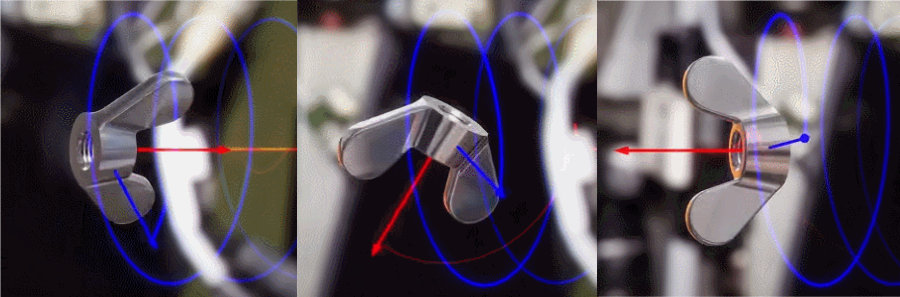
\includegraphics[width=0.9\textwidth]{dzhani.jpg}
\end{center}
   \caption{រូបភាពបង្ហាញអំពីឥទ្ធិពេលរបស់ Dzhanibekov \cite{28}។}
\label{fig:10}
\end{figure*}

គោលការណ៍ដែលនៅក្រោយការប្រែប្រួលយ៉ាងឆាប់រហ័សនៃអ័ក្សបង្វិលរបស់ផែនដីគឺផ្អែកលើរូបវិទ្យានៃការបង្វិលរបស់អង្គធាតុ។ ឧទាហរណ៍ជាក់ស្តែងដែលតំណាងឱ្យរឿងនេះគឺ «ឥទ្ធិពល Dzhanibekov» (Dzhanibekov effect) ដែលត្រូវបានរកឃើញដោយអវកាសយានិករុស្ស៊ីឈ្មោះ Vladimir Dzhanibekov។ \cite{37} ហើយបង្ហាញក្នុងរូបទី \ref{fig:10}។ អ័ក្សណាមួយដែលមិនអាចបង្វិលបានល្អក្នុងចំណោមអ័ក្សសំខាន់ 3 នៃសន្ទុះធ្ងន់ (principal axes of inertia) នោះវានឹងមិនអាចរក្សាលំនឹងអ័ក្សបង្វិលឲ្យនៅថេរបានឡើយ។ បើអ័ក្សមួយវិលជិតអ័ក្សសំខាន់ទីពីរ វានឹងប្រឈមនឹងការផ្លាស់ប្តូរទិសដៅបង្វិលភ្លាមៗ។ ទោះបីនេះមិនមែនជាអ្វីដែលយើងជឿថាកើតមានក្នុងអំឡុងពេលផែនដីប្តូរទិសបង្វិលភ្លាមៗក៏ដោយ ចំណុចសំខាន់គឺថាប្រសិនបើគ្មានកម្លាំងបង្ខំពីខាងក្រៅទេនោះអ្វីដែលអាចពន្យល់ពីការផ្លាស់ប្តូរទិសដៅភ្លាមៗដែលផែនដីវិល​នោះគឺមកពីមានច្បាប់រូបវិទ្យានៃការរង្វិលផ្សេងទៀត។​

ជាក់ស្តែងទៅ ផែនដីប្រហែលជាមិនបានជួបប្រទះនឹងឥទ្ធិពល Dzhanibekov (Dzhanibekov effect) ដែលមានភាពសាមញ្ញនិងស្មើគ្នាទេ។ បើរឿងនេះជារឿងពិត ពួកយើងប្រហែលជាអាចចាប់បាននូវការផ្លាស់ប្តូរការរង្វិលរបស់ផែនដី (Earth’s rotational axis)ជាបន្តបន្ទាប់ក្នុងរយៈពេលកន្លងមកហើយ។ផ្ទុយទៅវិញ ពួកយើងជឿថា ផែនដីធ្លាប់ឆ្លងកាត់រយៈពេលមួយដែលមានការកាត់ផ្តាច់ភ្លាមៗនៅរចនាសម្ព័នរូបវិទ្យារបស់វា​ដែលស្ថានភាពនេះនាំឲ្យឈានទៅដល់ការផ្ដាច់ចេញពីគ្នារវាងផ្នែកបង្វិលខាងក្រៅ (outer rotational – សែលក្រាស់ និងស្រទាប់ mantle) និង ផ្នែកបង្វិលខាងក្នុង (inner rotational bodies – ស្រទាប់ស្នូល core) នេះចង់មានន័យថា ផ្នែកខាងក្រៅនៃផែនដីចាប់ផ្តើមបង្វិលដោយឡែកពីផ្នែកខាងក្នុង ផែនដីមិនបង្វិលរួមដូចមុនទៀតទេ។ច្បាប់អំពីការរក្សាលំនឹង (law of conservation of angular momentum) បានបញ្ជាក់ថា​បើគ្មានឥទ្ធិពលពីខាងក្រៅផែនដី​ផែនដីមិនអាចផ្លាស់ប្តូរអ័ក្សបង្វិលរបស់ខ្លួនដោយភ្លាមៗបានទេ​ដូច្នេះការបែកចេញពីគ្នារវាងផ្នែកបង្វិលខាងក្រៅ និងផ្នែកបង្វិលខាងក្នុងរបស់ផែនដី គឺជាហេតុផលមួយក្នុងចំណោមមូលហេតុពីរ​បីប៉ុណ្ណោះ ដែលអាចបណ្តាលឲ្យមានការបង្វិលប្តូរទិសដ៏ភ្លាមៗរបស់ផែនដី។

ដំណើរការពិសេសដែលជួយជំរុញឲ្យកើតមានការរំខានផ្នែកខាងក្នុងនៃផែនដីត្រូវគេជឿថាជាការផ្លាស់ប្តូរស្ថានភាពក្នុងរចនាសម្ព័ន្ធធាតុដែកដែលជាស្នូលផែនដី (រូបទី \ref{fig:11})។ ស្នូលខាងក្នុងរបស់ផែនដីមានសមាសភាពជាដែកថែបដែលមានរូបរាងជាដុំដែកបិទជិតមានមុំប្រាំមួយ (hexagonal close-packed Iron​ឬ​HCP Fe) \cite{141}។ នៅពេល Hcp-Fe ត្រូវបម្លែងទៅជាលោហៈធាតុរាវ​វាបានបញ្ជេញថាមពលស្រូបទាញ​ហើយត្រូវបានជ្រាបចូលទៅក្នងស្រទាប់ទីពីរដែលជាស្រទាប់បន្ទាប់ពីស្នូលផែនដី។ ការផ្លាស់ប្តូរស្ថានភាពនេះធ្វើឲ្យកាត់បន្ថយសមត្ថភាពស្នូលរបស់អេឡិចត្រូម៉ាញ៉េទិក នាំឲ្យដែនម៉ាញ៉េទិករបស់ផែនដីមានកម្លាំងខ្សោយ រួចវាក៍បញ្ចេញកម្តៅ បង្កើតឲ្យមានរចនាសម្ព័ន្ធកម្លាំងរមៀលបន្តយឺតតំបន់ធំមួយ(LLVP)(រូបទី \ref{fig:12}) \cite{38} នៅក្នុងស្រទាប់មេនថល ហើយចលនានេះបានដុតកម្តៅផ្ទៃផែនដីតាមរយៈបាតសមុទ្រ។និន្នាការទាំងពីរនេះត្រូវបានកត់ត្រាដោយលម្អិតនៅក្នុងសតវត្សថ្មីៗនេះ ហើយត្រូវបានពិភាក្សាបន្ដក្នុងផ្នែកខាងក្រោយនៃអត្ថបទស្រាវជ្រាវនេះ។

\begin{figure*}[t]
\begin{center}
% \fbox{\rule{0pt}{2in} \rule{.9\linewidth}{0pt}}
\includegraphics[width=1\textwidth]{layers.jpg}
\end{center}
   \caption{ការបង្ហាញពីដំណើរការ​ក្នុងផ្ទៃផែនដី​ដែលនាំឲ្យមានការប្ដូរទិសដៅ ECDO \cite{129}.}
\label{fig:11}
\end{figure*}


\begin{figure}[t]
\begin{center}
% \fbox{\rule{0pt}{2in} \rule{0.9\linewidth}{0pt}}
   \includegraphics[width=1\linewidth]{llvp.jpg}
\end{center}
   \caption{រូបភាពលម្អិតនៃ LLVP នៅក្រោមអាហ្វ្រិកខាងត្បូង \cite{28}.}
\label{fig:12}
\label{fig:onecol}
\end{figure}

ដំណើរការដូចគ្នានេះនៅផ្នែកខាងក្នុងនៃផែនដីបានកើតឡើងទៅវិញទៅមក ហើយវាក៏ត្រូវបានគេជឿដែរថានេះជាមូលហេតុនាំឲ្យផែនដីវិលត្រឡប់ទៅស្ថានភាពបច្ចុប្បន្នវិញក្នុងរយៈពេលមិនយូរបន្ទាប់ពីការប្តូរប៉ូលនៃដែនម៉ាញ៉េទិក (flip) បានកើតឡើង។

\section{ភស្ដុតាងដែលអាចឲ្យដឹងថាការប្ដូរទិសប៉ូលនៃផែនដី(Earth flip)នឹងអាចកើតមានឆាប់ៗនេះ}

មានហេតុផលមូលដ្ឋានសំខាន់ដែលធ្វើឲ្យយើងជឿថា ឥឡូវនេះយើងកំពុងនៅជិតចំណុចនៃការប្ដូរទិសប៉ូលនៃផែនដី(Earth flip) ម្តងទៀត។​អស់រយៈពេលពីរបីពាន់ឆ្នាំមកហើយដែលគ្រោះមហន្តរាយទឹកជំនន់មិនបានកើតឡើង ហើយតាមកំណត់ត្រាប្រវត្តិសាស្ត្របានបង្ហាញថាគ្រោះធម្មជាតិតែងតែកើតឡើងរាល់ពីរបីពាន់ឆ្នាំម្តង។ទិន្នន័យមានសារសំខាន់បំផុតដែលគាំទ្រថាមាននឹងមានការប្ដូរទិសប៉ូលនៃផែនដីជិតកើតឡើង គឺផ្អែកលើទិន្នន័យម៉ាញេទិចភូមិសាស្ត្របច្ចុប្បន្ន​ដែលទិន្នន័យនេះចង្អុរបង្ហាញថា​ដែនម៉ាញេទិចភូមិសាស្ត្ររបស់ផែនដី (Earth’s geomagnetic field) កាន់តែចុះខ្សោយក្នុងរយៈពេលប្រហែល2,000ឆ្នាំចុងក្រោយនេះ។ការចុះខ្សោយនេះបានកើនល្បឿនឡើងវិញយ៉ាងឆាប់រហ័ស ហើយបានឈានដល់ចំណុចដែលគួរឱ្យព្រួយបារម្ភក្នុងពេលពីរបីទសវត្សរ៍ចុងក្រោយនេះ។


រូបភាពបានបង្ហាញក្នុងរូបទី\ref{fig:14} គឺជាដែនម៉ាញ៉េទិកនៃផែនដីក្នុងឆ្នាំ​1950​និង​2025 \cite{125,126}.ដូចដែលបានឃើញក្នុងរូបដែនម៉ាញ៉េទិកបានចុះខ្សោយយ៉ាងខ្លាំង។ 

វីធីវាស់វែងមួយទៀតសម្រាប់ដែនម៉ាញេទិចភូមិសាស្ត្រដែលកំពុងចុះខ្សោយ គឺមើលលើទីតាំងនៃដែនម៉ាញេទិកភូមិសាស្ត្រនៅប៉ូលខាងជើង។ (Figure \ref{fig:13}). ដែនម៉ាញេទិកភូមិសាស្ត្រនៅប៉ូលខាងជើងមានប្រវត្តិស្ថិតនៅតំបន់អាកទិកនៃប្រទេសកាណាដា។ប៉ុន្តែដែនម៉ាញេទិកប៉ូលខាងជើងបានចុះខ្សោយយឺតៗក្នុងរយៈពេលប៉ុន្មានសតវត្សចុងក្រោយនេះ ហើយបានកើនល្បឿនយ៉ាងខ្លាំងក្នុងរយៈពេលពីរបីទសវត្សរ៍ចុងក្រោយ។ បច្ចុប្បន្នវាកំពុងផ្លាស់ទីយ៉ាងលឿនទៅត្រឹមតែប្រទេសរុស្ស៊ី ដោយល្បឿន 55 គីឡូម៉ែត្រក្នុងមួយឆ្នាំ។\cite{124}.

\begin{figure*}[t]
\begin{center}
% \fbox{\rule{0pt}{2in} \rule{.9\linewidth}{0pt}}
\includegraphics[width=0.9\textwidth]{saa.jpg}
\end{center}
   \caption{សេចក្ដីបង្ហាញអំពីដែនម៉ាញេទិកភូមិសាស្ត្រដែលកំពុងចុះខ្សោយនេះ ចាប់ពីឆ្នាំ 1590 ដល់ 2025។ ត្រូវបានគណនាដោយប្រើម៉ូដែល gufm1 និង IGRF-14។\cite{125,126}។}
\label{fig:14}
\end{figure*}

\begin{figure}[t]
\begin{center}
% \fbox{\rule{0pt}{2in} \rule{1\linewidth}{0pt}}
   \includegraphics[width=1\linewidth]{npw.jpg}
\end{center}
\caption{ទីតាំងនៃដែនម៉ាញេទិកភូមិសាស្ត្រប៉ូលខាងជើងចាប់ពីឆ្នាំ 1590 ដល់ 2025 ត្រូវបានបង្ហាញឲ្យឃើញការថយចុះរៀងរាល់ 5 ឆ្នាំម្តង។ \cite{142}.}
\label{fig:13}
\label{fig:onecol}
\end{figure}

\begin{figure}[t]
\begin{center}
% \fbox{\rule{0pt}{2in} \rule{1\linewidth}{0pt}}
   \includegraphics[width=1\linewidth]{ocean-highlight.jpg}
\end{center}
   \caption{អត្រាការឡើងកម្តៅនៃបាតសមុទ្រជម្រៅ ($>$2000 ម៉ែត្រ) ពីឆ្នាំ 1991 ដល់ 2010​វាត្រូវបានគូសដោយរង្វង់ក្រហម \cite{132}.}
\label{fig:15}
\label{fig:onecol}
\end{figure}

ដែនម៉ាញេទិករបស់ភពផែនដីត្រូវបានគេជឿថាត្រូវបានបង្កើតដោយថាមពលឌីណាម៉ូពីខាងក្នុង​ថាមពលឌីណាម៉ូកើតពីរង្វិលៗនៃចរន្តម៉ាក្ម៉ា (magma currents) ដែលកំពុងផ្លាស់ទីក្នុងស្រទាប់ទីពីរបន្ទាប់ពីស្នូលរបស់ផែនដី (Earth’s outer core) ហើយចលនារង្វិលនេះកើតដោយសារតែការបង្វិលរបស់ផែនដី។\cite{123}។ ការចុះខ្សោយនៃដែនម៉ាញេទិកភូមិសាស្ត្ររបស់ផែនដី គឺជាសញ្ញាមួយបង្ហាញពីការរំខាននៅក្នុងផ្នែកខាងក្នុងដ៍ជ្រៅនៃផែនដី។ ដោយយោងទៅតាមទ្រឹស្តី ECDO, ការរំខានទាំងនេះច្រានកំដៅចេញ ហើយចុងក្រោយនាំឱ្យបំបែករវាងស្រទាប់ mantle និងស្នូលផែនដី ដែលបណ្ដាលឱ្យផែនដីមានព្រឹត្តិការណ៍ផ្លាស់ប្តូរទិសនៃប៉ូលនៃដែនម៉ាញ៉េទិករបស់ផែនដី \cite{1}។

មានទិន្នន័យជាច្រើនបញ្ជាក់ពីសកម្មភាពកម្ដៅនៅខាងក្នុងផែនដី។ ការឡើងកម្តៅនៃផែនដីត្រូវបានដឹងដោយសារការកត់ត្រាអំពីសីតុណ្ហភាពដែលកំពុងកើនឡើងនៅលើផ្ទៃដីគោក និងផ្ទៃសមុទ្រ\cite{127,128} កម្រិតឧស្ម័នកាបូនឌីអុកស៊ីតក្នុងបរិយាកាស (CO₂) កំពុងកើនឡើងជាសមស្របជាមួយការកើនឡើងនៃចំហាយកម្ដៅ (heat plumes) របស់ផែនដី។ \cite{129,130} និងការថយចុះនៃផ្ទៃសមុទ្រទឹកកករបស់ពិភពលោក \cite{131}។ ទិន្នន័យបង្ហាញថាកម្រិត CO2 និងសីតុណ្ហភាពដែលកើនឡើងមិនមែនជាកត្តាមកពីសកម្មភាពរបស់មនុស្សទេ ប៉ុន្តែវាបណ្តាលយមកពីឥទ្ធិពលនៃស្នូលផែនដីដែលបញ្ចេញកម្ដៅ (exothermic core)។ \cite{129}។

គួរឱ្យសំខាន់បំផុតនោះ ការសិក្សាអំពីអត្រាកម្តៅក្នុងបាតសមុទ្រជម្រៅប្រហែល($>$2000 ម៉ែត្រ) បង្ហាញថា មិនត្រឹមតែសមុទ្រជ្រៅកំពុងក្ដៅឡើងទេ ថែមទាំងមានអត្រាក្ដៅឡើងខ្លាំងបំផុតនៅស្រទាប់អាប៊ីស៊ិល abyssalរបស់សមុទ្រដែលមានជម្រៅប្រហែល 4000ទៅ6000 ម៉ែត្រ)។ កម្តៅនៃបាតសមុទ្រដ៍ជ្រៅនេះមានទីតាំងជ្រៅជាង4000 ម៉ែត្រ \cite{132,129} ដែលវានឹងមិនអាចទៅរួចទេ ប្រសិនបើសមុទ្រនៅជម្រៅនេះត្រូវឡើងក្តៅដោយសារបរិយាកាសខាងលើ។ ទិន្នន័យបានបង្ហាញយ៉ាងច្បាស់ថា ការប្រែប្រួលអាកាសធាតុនិងដែនម៉ាញេទិកនៅបច្ចុប្បន្ននេះត្រូវបានរងឥទ្ធិពលដោយដំណើរការដែលស្ថិតនៅក្នុងស្នូលនៃផែនដី។ រូបភាព \ref{fig:15} បង្ហាញអត្រាឡើងកម្ដៅទឹកសមុទ្រដ៍ជ្រៅរបស់ពិភពលោកពីឆ្នាំ 1991 ដល់ 2010 \cite{132}។

\section{វិធីសាស្ត្រដែលបង្ហាញថាការប្តូរទិសប៉ូលរបស់ផែនដីជិតកើតឡើង}

\begin{figure}[b]
\begin{center}
% \fbox{\rule{0pt}{2in} \rule{1\linewidth}{0pt}}
   \includegraphics[width=1\linewidth]{saa-crop.jpeg}
\end{center}
   \caption{ការគណនាទិន្នន័យពីតំបន់អាត្លង់តិកខាងជើងដែលមានដែនម៉ាញេទិករបស់ផែនដីខ្សោយ អាចឲ្យគេកំណត់កាលបរិច្ចេទថាការប្តូរទិសប៉ូលនៃដែនម៉ាញ៉េទិករបស់ផែនដីអាចកើតមាននៅអំឡុងថ្ងៃទី 13 ខែមីនា ឆ្នាំ 2059។ \cite{125,126}។}
\label{fig:16}
\label{fig:onecol}
\end{figure}

ការព្យាករពេលវេលានៃការប្តូរទិសប៉ូលនៃដែនម៉ាញ៉េទិករបស់ផែនដីលើកក្រោយ គឺជាការងារដែលស្មុគស្មាញ។ បច្ចុប្បន្ន ម៉ូដែលល្អបំផុតដែលយើងមានសម្រាប់ការងារនេះ គឺផ្អែកលើដែនម៉ាញ៉េទិករបស់ផែនដីដែលមានទីតាំងនៅតំបន់ខុសប្រក្រតីនៅអាត្លង់ទិកខាងត្បូង (SAA)។ តំបន់នេះនៅលើអាត្លង់ទិកខាងត្បូង វាមានកម្លាំងដែនម៉ាញេទិកភូមិសាស្ត្រខ្សោយជាងគេ ហើយត្រូវបានកំណត់ថាជាតំបន់ដែលមានកម្លាំងវាលម៉ាញេទិកក្រោម 32,000 ណាណូតេស្លា (nanoteslas)\cite{135} ដែលជាតម្លៃកម្លាំងខ្សោយបំផុតនៅឆ្នាំ 1590។​ផ្ទៃដីនៃតំបន់ខុសប្រក្រតីអាត្លង់ទិកខាងត្បូង (South Atlantic Anomaly) បានកើនឡើងពី1ភាគរយនៃផ្ទៃដីក្នុងឆ្នាំ​1590​ឡើងដល់21ភាគរយក្នុងឆ្នាំ2025\cite{136}។

ដើម្បីទទួលបានការព្យាករណ៍មួយចំពោះពេលវេលាដែលផែនដីអាចនឹងប្តូរទិសប៉ូល ខ្ញុំបានផ្គូផ្គងទិន្នន័យអំពីផ្ទៃដីនៃតំបន់ខុសប្រក្រតីអាត្លង់ទិកខាងត្បូង (SAA) ជាមួយទ្រឹស្តីថាមពលមួយរបស់ចំណុចបំប្លែង (tipping point equation) ដែលវិធីសាស្ត្រនេះជាប្រព័ន្ធដ៍ស្មុគស្មាញដែលឆ្ពោះទៅរកការការផ្លាស់ប្តូរដោយភាពល្អិតល្អន់បំផុត​ហើយប្រព័ន្ធនេះអាចត្រូវបានឆ្លងកាត់ការផ្លាស់ប្តូរដែលលឿននិងភ្លាមៗបំផុត។ការគណនារបស់ខ្ញុំបានផ្តល់នូវកាលបរិច្ឆេទនៃចំណុចបំប្លែង (tipping point) ដែលបានព្យាករណ៍ថា នឹងកើតឡើងនៅថ្ងៃទី 13 ខែមីនា ឆ្នាំ 2059(រូបភាព \ref{fig:16})។ ការព្យាករណ៍នេះនឹងកាន់តែត្រឹមត្រូវ នៅពេលដែលផែនដីកាន់តែទៅជិតទៅដល់ពេលនៃការផ្លាស់ប្តូរដែនម៉ាញ៉េទិកនៃប៉ូលរបស់ផែនដី​ \cite{136}។**************************

រង្វាស់ផ្សេងៗទៀតសម្រាប់ទស្សទាយមានដូចជាការប្តូរទិសនៃអ័ក្សបង្វិលរបស់ផែនដី (rotational axis wander) អាកាសធាតុខុសប្រក្រតី (weather anomalies) និងទិន្នន័យពីការរញ្ជួយដីនិងភ្នំភ្លើង ក៏អាចជួយឲ្យការព្យាករណ៍បានកាន់តែសុក្រឹតអំពីពេលវេលាដែលនឹងកើតមាននូវការប្តូរទីតាំងនៃដែនម៉ាញ៉េទិករបស់ផែនដី(Earth flip) ម្តងទៀត។

\section{បញ្ជីរកាលបរិច្ឆេទដែលព្រឹត្តិការណ៍​ECDO​បានកើតឡើងពីអតីតកាល}

ទោះបីជាការកំណត់ពេលវេលាជាក់លាក់សម្រាប់ព្រឹត្តិការណ៍ ECDO ក្នុងអតីតកាលជាការលំបាកក្តី​ព្រឹត្តិការណ៍ ECDO កើតឡើងយ៉ាងតិច2លើក ក្នុងអំឡុងសម័យដែលជាយុគសម័យថ្មីដែលចាប់ផ្តើមតាំងពីប្រហែល 11,700 ឆ្នាំមុន គឺបន្ទាប់ពីសម័យទឹកកកចុងក្រោយ ហើយបន្តរហូតដល់សព្វថ្ងៃ(Holocene)។សូមចំណាំពីការថ្លែងរបស់អ្នកប្រវត្តិវិទូហេរូដូទូស (Herodotus) ដែលធ្លាប់និយាយពីអ្វីដែលអ្នកបួសអេហ្ស៊ីបបានប្រាប់គាត់ \textit{"ចាប់តាំងពីព្រះមហាក្សត្រដំបូងបំផុតរហូតដល់អ្នកបួសនៃហេហ្វីទុសដែលជាជំនាន់ស្តេចចុងក្រោយ មានសរុបចំនួន341ជំនាន់..ក្នុងរយៈពេលនោះ ពួកគេបាននិយាយថា ព្រះអាទិត្យបានផ្លាស់ទីពីទីកន្លែងដែលវាធ្លាប់រះបួនដង ហើយទីកន្លែងដែលព្រះអាទិត្យរះសព្វថ្ងៃគឺជាកន្លែងដែលវាបានលិចពីមុនពីរដង ហើយទីកន្លែងដែលវាធ្លាប់លិចមកពីមុនឥឡូវក៍វាបានរះនៅទីនោះពីរដងដែរ}\cite{111}។អ្នកប្រាជ្ញក្រិចឈ្មោះ​ផ្លាតូ​(Plato) និយាយថាបន្ទាប់ពីទឹកជំនន់ដែលបានលិចទ្វីបអាត្លង់ទិកអស់មួយថ្ងៃមួយយប់ កាលពីប្រហែល9,000 ឆ្នាំមុននេះ។ \textit{"តាំងពីមានទឹកជំនន់ជាច្រើនលើកច្រើនសារកើតឡើងមក អ្នកដែលនៅសល់ដោយរួចផុតពីគ្រោះថ្នាក់ទឹកជំនន់ព្រោះតែពួកគេគេចទៅនៅលើភ្នំ ពួកគេមិនបានយកចិត្តទុកដាក់លើសិល្បៈនៃការសរសេរទេ ហើយអស់ជាច្រើនជំនាន់ពួកគេបានព្យាយាមយ៉ាងពេញទំហឹងក្នុងការស្វែងរកមធ្យោបាយសម្រាប់រស់នៅ។"} \cite{112} ដែលនេះបញ្ជាក់ថា មានការប្តូរដែនម៉ាញ៉េទិករបស់ផែនដីច្រើនជាងពីរលើក តាំងពីបញ្ចប់សម័យយុគទឹកកកយ៉ាងហ្គឺទ្រីយ៉ាស់(Younger Dryas) ប្រហែលឆ្នាំកាលពី 9700 មុន គ.ស.។ ភស្តុតាងរូបវិទ្យាដែលត្រូវបានបង្ហាញក្នុងអត្តបទនេះ និងក្នុងការស្រាវជ្រាវរបស់ខ្ញុំ\cite{2} បានផ្ដល់ភស្តុតាងច្រើនគ្រប់គ្រាន់ដើម្បីគាំទ្រការពិពណ៌នារបស់លោកផ្លាតូ។

កាលបរិច្ឆេទមួយចុងក្រោយបំផុតសម្រាប់ព្រឹត្តិការណ៍ ECDO គឺនៅចន្លោះឆ្នាំ 2300 ដល់ 1600 មុនគ.ស។ គេបានកត់ត្រាពីកាលបរិច្ឆេទនៃព្រឹត្តិការណ៍សំខាន់ទាំងនោះដូចជា​ទឹកជំនន់ធំៗ (ទឹកជំនន់ឈ្មោះហ្គុនយូ \cite{113,114,115}, អូជីហ្គេស \cite{116,117}, ប៉េរូ \cite{118,119}, អ៊ិចស្សូដឺស \cite{120}) ព្រឹត្តិការណ៍នៃការបំផ្លាញ និងការបោះបង់ចោលនៃអរិយធម៌របស់សង្គមមនុស្សដូចជា (ព្រឹត្តិការណ៍មូហេនចូ​ដារ៉ូ \cite{121}, មីណូអាន​ក្រេត\cite{100,101}) និងព្រឹត្តិការណ៍មិនប្រក្រតីនៃរូបវិទ្យាដូចជា (ព្រឹត្តិការណ៍បូន \cite{122}, ព្រឹត្តិការណ៍ 4200​ឆ្នាំ \cite{90})។ ចាប់តាំងពីព្រឹត្តិការណ៍ទាំងនោះមក យើងមិនឃើញថាមានភស្តុតាងច្បាស់លាស់អំពីវិនាសកម្មធំៗផ្សេងទៀតដែលបានកើតឡើងនាពេលបច្ចុប្បន្ននេះឡើយ។

\section{សេចក្តីសន្និដ្ឋាន}

ប្រតិបត្តិការណ៍ណានូកគឺជាប្រតិបត្តិការស៊ើបការណ៍របស់សហរដ្ឋអាមេរិកក្នុងសម័យសង្គ្រាមត្រជាក់ ដើម្បីកំណត់ផែនទីរបស់តំបន់អាក់តិក និងឆ្នេរភាគខាងជើងរបស់សហភាពសូវៀត បន្ទាប់ពីសង្គ្រាមលោកលើកទីពីរ។ \cite{137}។ ក្នុងអំឡុងពេលស៊ើបអង្កេត ពួកគេបានរកឃើញថា ប៉ូលម៉ាញេទិចស្ថិតនៅភាគខាងជើងឆ្ងាយជាងទីតាំងដែលគេរំពឹងទុកប្រហែល 125 ទៅ200ម៉ាយ បើធៀបនឹងលទ្ធផលដែលរកឃើញពីការស្រាវជ្រាវមុនៗ។ ដូច្នេះ \textit{"ក្នុងចំណោមអ្នកវិទ្យាសាស្ត្ររបស់រដ្ឋាភិបាល មានសំណួរមួយបានផុសឡើងថា តើអ្វីទៅដែលនឹងកើតឡើង នៅពេលប៉ូលម៉ាញេទិច និងប៉ូលភូមិសាស្ត្រត្រួតគ្នា។ ដើម្បីឆ្លើយសំណួរនេះ នាយកគម្រោងគ្រប់គ្រងដោយលោកបណ្ឌិត​ផូល​អេ​របស់ក្រុមហ៊ុនសហប្រតិបត្តិការ​រេនដ៍បានចុះកិច្ចសន្យាដើម្បីធ្វើការសិក្សាស្រាវជ្រាវដោយប្រើប្រាស់គម្រូនៃផែនដីដែលបង្កើតពីស្រទាប់ស្របជុំគ្នា វាមានស្រទាប់ខាងក្នុងតំណាងឲ្យស្នូលដែករាវដែលមានផ្ទុកអគ្គិសនីនិងម៉ាញេទិច​ស្នូលដែករាវដែលមានផ្ទុកអគ្គិសនីនិងម៉ាញេទិចរបស់ផែនដី ដែលអ័ក្សរបស់វាបង្កើតប៉ូលម៉ាញេទិក។តាមរយៈការធ្វើតេស្តឡើងវិញបានបង្ហាញថា ប៉ូលម៉ាញេទិក នៅពេលដែលវាឈានទៅជិតប៉ូលភូមិសាស្រ្ត នោះ ប៉ូលម៉ាញេទិកនឹងចាប់ផ្តើមមានល្បឿននៃការរួមជាមួយគ្នាបានលឿនជាងមុន ដូចជាត្រូវបានទាញទៅរកប៉ូលភូមិសាស្រ្តដោយកម្លាំងសេន្ដ្រីប៊ូតាល់ហើយចាប់ផ្តើមលោតរួមជាមួយប៉ូលភូមិសាស្រ្ត។
ប៉ុន្តែជំនួសឱ្យដំណើរការរួមគ្នារវាងប៉ូលទាំងពីរ ប៉ូល“ម៉ាញេទិក”ត្រូវបានគេឃើញថា“បង្វិលផ្ទុយ”យ៉ាងឆាប់រហ័សនៅជុំវិញប៉ូល“ភូមិសាស្ត្រ” បន្ទាប់មកវាបានបង្វិលចេញទៅទិសខ្សែអេក្វាទ័រជាមួយនឹងកម្លាំងប៉ះពាល់សេន្ទ្រីហ្វូ (centrifugal force) ហើយចាប់ផ្ដើមបញ្ចប់នៅទីតាំងមួយ ដែលជាទីតាំងដែលអ័ក្សទាំងពីរនោះមានភាពខុសគ្នាប្រហាក់ប្រហែល 89 ដឺក្រេ។បន្ទាប់ពីមានការផ្លាស់ប្តូរដែនម៉ាញ៉េទិករបស់ប៉ូល​អ័ក្សនឹងចាប់ផ្តើមបង្វិលត្រឡប់មកជារួមវិញក្នុងរយៈពេលយូរម្ដងៗ"} \cite{138,139}។

បន្ទាប់មក \textit{"នៅក្នុងសន្និសិទមួយរបស់សមាជិក​Major White បានចូលរួមនៅផេនតាហ្គន​(Penthagon)ដើមឆ្នាំ 1948 អ្នកវិទ្យាសាស្ត្របានពិភាក្សាអំពីភាពសមស្របក្នុងការប្រាប់សាធារណជនអំពីព្រឹត្តិការណ៍ប្តូរដែនម៉ាញ៉េទិករបស់ផែនដី។ គ្មានអ្នកវិទ្យាសាស្ត្រណាមួយព្រមរក្សាការសម្ងាត់ពីពត៌មាននេះពីសាធារណជនទេ ប៉ុន្តែម្យ៉ាងទៀតពួកគេក៏មិនទាន់យល់ស្របគ្នាផងដែរអំពីរបៀបបង្ហាញពត៌មាននេះទៅកាន់សាធារណជន។ ចំណេះដឹងអំពីព្រឹត្តការណ៍មហន្តរាយនេះ មួយចំនួនគិតថា អាចនាំមានការបំផ្លាញសរសៃឈាមរបស់សង្គមដូចជាសីលធម៌និងគុណធម៌។ ការភ័យខ្លាចរបស់ប្រជារាស្ត្រគឺមិនត្រូវបានបង្ហាញទេ នៅដើមឆ្នាំ 1950 បើទោះបីជាពត៌មានអំពីផែនដីប្តូរប៉ូលម៉ាញ៉េទិកបានបង្ហោះក្នុងកាសែតនិងទស្សនាវដ្តីមួយ ហើយក៍គ្មានការឆ្លើយតបពីសាធារណជនក្នុងរបៀបណាមួយគួរឲ្យភ្ញាក់ផ្អើលឡើយ"} \cite{138,139}។

ហេតុអ្វីបានជា​យើងមិនយកចិត្តទុកដាក់អំពីរឿងនេះ? មានហេតុផលច្រើនគ្រប់គ្រាន់អោយយើងជឿថាភពផែនដីធ្លាប់ប្តូរប៉ូលម៉ាញ៉េទិកពិតមែន។ អត្តបទនេះរួមទាំងផ្នែកទីពីររបស់វា ផ្ដល់សង្ខេបខ្លីនៃភស្តុតាងពីភស្តុតាងជាច្រើនដែលបង្ហាញថាវាជាបញ្ហា​ដូចជារឿងទឹកជំនន់ជុំវិញពិភពលោក វាលអំបិលនិងហ្វូស៊ីលដែលគ្រប់ដណ្តប់លើទ្វីប ជម្រកក្រោមដីពីបុរាណ សត្វដែលនៅសល់់ និងផ្ទៃដីភូមិសាស្ត្រដែលរងគ្រោះ។តើមិនអាចជាករណីដែល ពេលខ្លះៗ ពិភពលោកបានប្តូរប៉ូលម៉ាញ៉េទិក ឬ? ដើម្បីឲ្យទ្វីបត្រូវបានបំផ្លាញអស់ រួចមនុស្សត្រូវត្រឡប់ទៅចំណុចចាប់ផ្ដើមវិញ ដូចជាសម័យថ្ម ហើយធ្វើឲ្យកំណត់ត្រាបុរាណសំបូរតែរឿងរ៉ាវគ្រោះមហន្តរាយធម្មជាតិ?ប្រសិនបើដូច្នេះ ការការពារមិនអោយវិបត្តិនេះកើតឡើងម្ដងទៀតក៏អាចជាកិច្ចការសំខាន់បំផុតរបស់មនុស្សជាតិផងដែរ។

ជាចុងក្រោយ ខ្ញុំនឹងទុកឲ្យអ្នកអានអំពីរឿងមួយក្នុងសៀវភៅទីមូស(Timaeus) ដែលប្លាតុងបានសរសេរពីការសន្ទនារវាងលោកមន្រ្តីសូឡូន  និងអ្នកបួសអេហ្ស៊ីប \cite{140}: \textit{"ហើយក្នុងឱកាសមួយ ពេលសូឡុន(Solon) ប្រាថ្នាចង់អោយពួកគេចាប់ផ្តើមពិភាក្សាអំពីប្រវត្តិសាស្រ្តបុរាណ គាត់បានព្យាយាមនិយាយអំពីទំនៀមទម្លាប់បុរាណបំផុតរបស់ពួកយើង ដែលទាក់ទងនឹងផូរណេអ៊ុស (Phoroneus)និងនិយោប៊ី (Niobe)ដែលត្រូវបាននិយាយថាជាបុរសដំបូងបង្អស់ ​ហើយគាត់បន្តនិយាយអំពីរឿងព្រេងនៃឌឺខាលីអុន និង ភៀរ៉ាបន្ទាប់ពីទឹកជំនន់ ហើយបញ្ជាក់ពីរបៀបដែលពួកគាត់បានរស់រានមានជីវិតរួចផុតពីវាហើយ​ដោយការរាប់ចំនួនឆ្នាំដែលព្រឹត្តិការណ៍នានាបានកើតឡើង គាត់បានព្យាយាមគណនាឱ្យបានច្បាស់អំពីរយៈពេលនៃកាលៈទេសៈនីមួយៗអាចនឹងកើតមានម្តងទៀត។
នៅពេលមួយមានអ្នកបួសដែលមានអាយុវែងបំផុតម្នាកបាននិយាយ​អូ សូឡុន សូឡុន! ពួកក្រិកមិនមែនជនជាតិចំណាស់បំផុតនោះទេ  ហើយក៍គ្មានអ្វីដែលហៅថាក្រិកដែលមានអាយុកាលដ៍យូរលង់ណាស់មកហើយដែរ។​ពេលលឺបែបននេះ គេចាប់ផ្តើមសួរថា “តើលោកគ្រូមានប្រសាសន៍បែបនេះមានន័យថាម៉េច?” ខណៈបូជាចារ្យបានឆ្លើយថា “អ្នកទាំងអស់គ្នាគឺជាបុគ្គលវ័យក្មេងព្រោះតែមានដួងព្រលឹងដែលនៅក្មេង ព្រោះនៅទីនេះអ្នកមិនបានអានសិល្បៈណាដែលចាស់ៗមកពីប្រវត្តិសាស្ត្រចាស់ៗទេ អ្នកក៏មិនមានវិទ្យាសាស្ត្រដែលមានវ័យចំណាស់ផងដែរ។ នេះជាមូលហេតុដែលនៅតែមានការបំផ្លាញមនុស្សជាច្រើនដំណាក់កាលទៀតដូចជាមានភ្លើងនិងទឹក គ្រាន់តែដោយរបៀបផ្សេងៗគ្នា។ រឿងពិតដែលនិយាយនៅក្នុងប្រទេសអ្នករបស់ដូចជារឿង Phaethon ដែលជាកូនរបស់ Helios ព្រោះគេមិនអាចដឹករទេះសេះបានល្អដូចឪពុករបស់គេទេ ហេតុនេះគេបានធ្វើឲ្យឆេះផែនដីទាំងមូលដោយអចេតនា ហើយចុងក្រោយគេក៏បានរងគ្រោះស្លាប់ដោយរន្ទះបាញ់ រឿងនេះជារឿងនិទាន ប៉ុន្តែផ្អែកលើផ្លាស់ប្តូរទីតាំងនៃផ្ទៃមេឃដែលត្រូវធ្វើឲ្យផែនដីក្រឡាបចាក់​ហើយបំផ្លាញគ្រប់យ៉ាងនៅលើផែនដីដោយភ្លើងដ៍សណ្ធោសន្ធៅ។ ដោយហេតុនេះអ្នករស់នៅលើភ្នំនិងកន្លែងខ្ពស់ហើយស្ងួតនឹងប្រឈមនឹងការបាត់បង់ជីវិតជាងអ្នកស្ថិតនៅជិតទន្លេឬសមុទ្រ។ ចំពោះករណីរបស់យើងជាអ្នកទន្លេនីល​ការអាចគេចផុតពីគ្រោះមហន្តរាយទឹកជំនន់គឺការរស់នៅកន្លែងខ្ពស់ៗ។ ហើយនៅពេលដែលក្រុមតំណាងព្រះមកសម្អាតផែនដីចេញដោយទឹកភ្លៀង អ្នកគង្វាលចៀមទាំងឡាយដែលនៅលើភ្នំត្រូវបានរួចពីស្លាប់​ប៉ុន្តែអ្នកនៅក្នុងទីក្រុងនានានៃដែនដីរបស់អ្នក ត្រូវបានទឹកគួចចូលទៅក្នុងសមុទ្រដោយស្ទឹងនានា។ ចំណែកនៅក្នុងប្រទេសរបស់ពួកយើង ទឹកមិនដែលហូរចុះពីលើមកពន្លិចដីដូច្នេះទេទាំងពេលនោះនិងពេលណាផ្សេងទៀត ផ្ទុយទៅវិញទឹកតែងតែជ្រៀបពីក្រោមដីមកវិញដោយធម្មជាតិ។​ហេតុនេះហើយអ្វីៗដែលនៅសេសសល់នៅទីនេះ ត្រូវបានរាប់ថាជាវត្ថុបុរាណបំផុត។ ការពិតគឺនៅគ្រប់ទីកន្លែងដែលមិនក្តៅខ្លាំងពេក ឬ ត្រជាក់ខ្លាំងពេកមិនឲ្យមនុស្សរស់នៅបានទេ តែនៅតែមានពូជមនុស្សមួយស្ថិតនៅទីនោះជានិច្ចមិនថាតិចឬច្រើន។ហើយបើមានព្រឹត្តិការណ៍ណាមួយដែលមានតម្លៃ ឬ វិសេសឬធំធេង ឬសម្រុកចេញមកតាមរបៀបណាក៏ដោយ មិនថាកើតឡើងនៅប្រទេសរបស់អ្នក ប្រទេសរបស់ពួកយើង ឬនៅកន្លែងផ្សេងទៀតដែលពួកយើងបានដឹងតាមរបាយការណ៍ក៏ដោយ ព្រឹត្តិការណ៍ទាំងអស់នោះត្រូវបានកត់ត្រាចាប់តាំងពីបុរាណ និងរក្សាទុកនៅក្នុងប្រាសាទរបស់ពួកយើង។ចំណែកប្រជាជនរបស់អ្នក និងអ្នកដទៃវិញ ដែលទើបតែចាប់ផ្តើមបង្កើតនៅអក្សរ និងសិល្បៈនានាដែលចាប់ផ្តើមបង្កើតជាសង្គមមនុស្សបែបទំនើប​ហើយពេលដែលកន្លងហួសទៅមួយរយៈពេល នោះក៍មានគ្រោះអាក្រក់ដូចជាជំងឺរាតត្បាតកើតឡើង​ពេលទឹកជំនន់មកពីលើមេឃហូរចុះមកលើប្រជាជនរបស់អ្នកម្តងទៀត វាបានបំផ្លាញអ្នកទាំងអស់ លើកលែងតែអ្នកដែលមិនសូវមានការអប់រំ និងគ្មានវប្បធម៌។ ដូច្នេះអ្នកត្រូវក្លាយជាមនុស្សថ្មីឡើងវិញជារឿយៗ ដោយគ្មានចំណេះដឹងអំពីអ្វីៗដែលបានកើតឡើងនៅក្នុងប្រទេសនេះ ឬប្រទេសរបស់អ្នកក្នុងសម័យបុរាណឡើយ។ច្បាស់ណាស់ ប្រវត្តិជនជាតិនានាដែលអ្នក​(សូឡូន) ទើបនិយាយកន្លងមកអំពីប្រជាជនក្នុងប្រទេសរបស់អ្នក វាមានតម្លៃតិចជាងរឿងរបស់កុមារ ពីព្រោះដំបូងអ្នកចាំបានតែទឹកជំនន់ធំមួយគត់ ប៉ុន្តែជំនន់ទឹកធំនោះបានកើតមានមកហើយជាច្រើនដងកាលពីមុនមក​បន្ទាប់មកអ្នកក៏មិនដឹងថាជនជាតិដែលមានគុណធម៌ខ្ពង់ខ្ពស់បំផុត និងមានភាពល្អឥតខ្ចោះបំផុតក្នុងចំណោមមនុស្ស បានកើតនៅលើដីដែលអ្នកកំពុងរស់នៅទេ​ឥឡូវនេះអ្នកផ្ទាល់ព្រមទាំងទីក្រុងទាំងមូលរបស់អ្នកដែលមាននៅបច្ចុប្បន្នត្រូវបានចេញមកពីពូជដើមទាំងនោះ នេះគឺបណ្តាលមកពីគ្រាប់ពូជតូចមួយដែលនៅសល់។ ប៉ុន្តែអ្នកមិនបានសង្កេតឃើញអំពីរឿងនេះទេ ពីព្រោះជាច្រើនជំនាន់ អ្នកដែលនៅសល់ពីការស្លាប់ពីមុនពួកគេបានស្លាប់អស់ ដោយពួកគេមិនមានសមត្ថភាពក្នុងការរៀបរាប់ពីខ្លួនរបស់ពួកគេតាមរយៈការសរសេរ។ ATTACH HERE ជាការពិតមែនសូឡុន​នៅមុនពេលការបំផ្លាញដ៏ធំបំផុតដោយទឹកបានកើតឡើង រដ្ឋអាថែន (Athenian State)កាលពីមុនធ្លាប់ជារដ្ឋដ៏ក្លាហានបំផុតក្នុងសង្គ្រាម ហើយមានរចនាសម្ព័ន្ធល្អបំផុតគ្រប់វិស័យផងដែរ។ គេបាននិយាយថារដ្ឋនេះបានកាន់កាប់ស្នាដៃសិល្បៈដ៏អស្ចារ្យបំផុត និងប្រព័ន្ធគ្រប់គ្រងរដ្ឋាភិបាលដ៏ខ្ពង់ខ្ពស់បំផុត បើប្រៀបធៀបនឹងជនជាតិណាមួយនៅក្រោមមេឃ ដែលពួកយើងធ្លាប់បានឮអំពីវា។"}។

អ្នកបួសដដែលនេះបានប្រាប់សូឡូនអំពីអធិរាជ្យបុរាណរបស់អាត្លង់ទិកផងដែរ៖ \textit{"មកដល់ពេល កន្លែងដែលពួកយើងកំពុងនិយាយអំពីគឺវាស្រដៀងទៅនឹងឈូងសមុទ្រ វាជាអាងទឹកតូចមួយដែលមានផ្លូវទឹកចូលតូច តែមិនមែនជាសមុទ្រពិតទេ។ ប៉ុន្តែកន្លែងដែលឆ្ងាយមួយទៀត វាជាសមុទ្រពិតប្រាកដ វាធំទូលាយនិងអស្ចារ្យហើយដីដែលព័ទ្ធជុំវិញសមុទ្រនោះធំណាស់​បើយោងតាមអត្ថន័យពេញលេញនិងពិតប្រាកដ​វាសមស្របណាស់ក្នុងការហៅថាជាទ្វីប។ឥឡូវនេះ នៅលើទ្វីបអាត្លង់ទិកមានសហព័ន្ធរបស់ព្រះមហាក្សត្រ ដែលមានអំណាចអស្ចារ្យនិងអស្ចារ្យយ៉ាងខ្លាំង ដែលមន្ត្រីរដ្ឋធំៗនីមួយៗត្រូវបានគ្រប់គ្រងកោះទាំងមូល ហើយក៏គ្រប់គ្រងទឹកដីជាច្រើនផ្សេងទៀតផងដែររួមទាំងផ្នែកខ្លះនៃទ្វីបផងដែរ បន្ថែមពីនេះទៀតតាមរយៈផ្លូវភ្ជាប់រវាងសមុទ្រ ពួកគេក៏បានគ្រប់គ្រងលើប្រទេសលីប៊ីយ៉ាហូតដល់អេហ្ស៊ីប និងលើទ្វីបអឺរ៉ុបរហូតដល់ទីរូយ៉ានៀផងដែរ។​ដូច្នេះកងទ័ពនេះបានរួមបញ្ចូលគ្នាទាំងអស់ បានព្យាយាមវាយតែម្តងឲ្យឈ្នះ​ដើម្បីដាក់ឲ្យប្រទេសរបស់អ្នក និងប្រទេសរបស់ពួកយើង និងដែនដីទាំងមូលនៅខាងក្រោមការគ្រប់គ្រងរបស់ខ្លួន។​សូឡូនហើយនៅពេលនោះហើយ​ជាពេលដែលសភាពជាអ្នកក្លាហាន និងអំណាចរបស់រដ្ឋអ្នក បានបង្ហាញខ្លួនយ៉ាងឆ្នើមចំពោះពិភពលោកទាំងមូល។​ដោយសារតែរដ្ឋរបស់អ្នកបានលេចធ្លោលើសគេដោយសារសេចក្តីក្លាហាន និងសិល្បៈសង្គ្រាមទាំងអស់ ពេលខ្លះក៍បានដើរតួជាអ្នកដឹកនាំរបស់ក្រិកទាំងមូល និងពេលខ្លះក៏បានឈរតែម្នាក់ឯង​ព្រោះតែបានបង្ក្រាបកងទ័ពដទៃអស់។ បន្ទាប់ពីពេលប៉ះពាល់នឹងគ្រោះអាក្រក់ដ៏សាហាវ ពួកគេបានវាយបំបែកពួកជនឈ្លានពាន និងបានបញ្ចប់សង្គ្រាមជាមួយនឹងជ័យជម្នះ ដោយសារតែសកម្មភាពទាំងនេះ ពួកគេបានជួយសង្គ្រោះអ្នកដែលជាទាសករ​អ្នកដែលរស់នៅក្នុងព្រំដែននៃហេរ៉ាឃ្លេស (Heracles) ឲ្យមានសេរីភាពមកវិញ។"}។

\section{សេចក្តីថ្លែងអំណរគុណ}

ខ្ញុំសូមអរគុណលោក Ethical Skeptic ដែលជាអ្នកនិពន្ធដើមនៃសន្និដ្ឋានលើព្រឹត្តិការណ៍ECDO ដែលបានសរសេរបញ្ជប់នូវទ្រឹស្តីថ្មីដែលពោរពេញដោយអត្ថន័យ និងធ្វើការចែករំលែកទូទាំងពិភពលោក។ បទនិពន្ធទាំងបីផ្នែករបស់គាត់ \cite{1} បានរក្សានូវស្នាដៃដើមដ៍សំខាន់អំពីទ្រឹស្តី Exothermic Core-Mantle Decoupling Dzhanibekov Oscillation (ECDO) និងមានព័ត៌មានច្រើនជាងនូវអ្វីដែលខ្ញុំបានលើកឡើងក្នុងអត្តបទនេះ។

អរគុណចំពោះអានឃិត(Ankit), ដែលបានរៀបចំប្រមូលផ្ដុំទិន្នន័យអំពីគ្រោះមហន្តរាយធម្មជាតិក្នុងតារាង1 ។

ហើយពិតណាស់ យើងសូមអរគុណយ៉ាងខ្លាំងដល់អ្នកឆ្នើមៗពីមុនមក ដូចជាអ្នកដែលបានធ្វើការស្រាវជ្រាវ និងស្វែងរកយ៉ាងលំបាក ដើម្បីឲ្យស្នាដៃនេះអាចកើតមានឡើងបាន។ ពួកគេបានជួយនាំចំណេះដឹង និងការយល់ដឹងមកឲ្យមនុស្សជាតិ។

\clearpage
\twocolumn

\section{រូបភាពបន្ថែម}

\begin{figure}[H]
\begin{center}
% \fbox{\rule{0pt}{2in} \rule{1\linewidth}{0pt}}
   \includegraphics[width=1\linewidth]{wave.jpg}
\end{center}
   \caption{រូបភាពបង្ហាញពីភាពខុសគ្នានៃខ្សែរកោងនៃការកើនកម្ដៅនៅជ្រលងសមុទ្រដ៏ជ្រៅនិងជ្រៅខ្លាំង បើប្រៀបធៀបនឹងខ្សែកោងធម្មតានៃការកើនកម្ដៅសមុទ្រដែលមានទំនាក់ទំនងជាមួយបរិយាកាស។ភាពខុសគ្នានៃការកើនកម្ដៅសរុប ត្រូវបានយកពី NOAA\cite{147}​ខណៈដែលការចែកចាយនៃកម្ដៅនៅជ្រលងជ្រៅខ្លាំងនៃសមុទ្រ ត្រូវបានយកពីសិក្សារបស់ Desbruyères\cite{132}​ហើយការប្រមូលទិន្នន័យ និងការបង្ហាញជារូបភាព ត្រូវបានអនុវត្តដោយលោក Ethical Skeptic។\cite{27}។}
\label{fig:19}
\label{fig:onecol}
\end{figure}

\begin{figure}[H]
\begin{center}
% \fbox{\rule{0pt}{2in} \rule{1\linewidth}{0pt}}
   \includegraphics[width=1\linewidth]{star-stone.jpg}
\end{center}
   \caption{កម្រិតទឹកសមុទ្របានបង្ហាញពីការកើនឡើង20ភាគរយ ក្នុងការប្រែប្រួលគម្លាតក្នុងរយៈពេល75ឆ្នាំ តាមតបន់63កន្លែង ដែលបញ្ជាក់ថា ល្បឿននៃចរន្តសមុទ្រកំពុងកើនឡើង។ការកើនឡើងបែបនេះនៃការប្រែប្រួលកម្រិតទឹកសមុទ្រត្រូវបានឃើញថាភ្ជាប់ជាមួយនឹង បញ្ចេញកំដៅដោយសមុទ្រ (ocean heat pulses) ដែលអាចបញ្ជាក់ថារឿងទាំងពីរនេះអាចបណ្តាលមកពីកំដៅកើតចេញពីជ្រលងក្រោមសមុទ្រ។\cite{28}។}
\label{fig:20}
\label{fig:onecol}
\end{figure}

\begin{figure*}[t]
\begin{center}
% \fbox{\rule{0pt}{2in} \rule{.9\linewidth}{0pt}}
\includegraphics[width=1\textwidth]{deepsea.jpg}
\end{center}
   \caption{បរិមាណឧស្ម័នកាបូនិច (CO₂) ក្នុងបរិយាកាស ត្រូវបានរកឃើញថាកើនឡើងយ៉ាងខ្លាំងជាប់ៗគ្នាក្នុងរយៈពេល45ឆ្នាំចុងក្រោយនេះ។ការកើនឡើងនេះ ប្រហែលជាបណ្តាលមកពីការកើនឡើងនៃសីតុណ្ហភាពសមុទ្រ។ប្រភព៖ NOAA (សេវាព័ត៌មានអាកាសធាតុអាមេរិក)។\cite{2,129}។}
\label{fig:21}
\end{figure*}
\begin{figure*}[t]
\begin{center}
% \fbox{\rule{0pt}{2in} \rule{.9\linewidth}{0pt}}
\includegraphics[width=1\textwidth]{sealevel.jpeg}
\end{center}
   \caption{ផ្ទៃក្រឡាសមុទ្រទឹកកក បានកាន់រួមតូចទៅក្នុងរយៈពេល45ឆ្នាំចុងក្រោយ ដោយសារដែនដីកំពុងក្ដៅ។ ប្រភព៖ ADS \cite{149}។}
\label{fig:22}
\end{figure*}

\begin{figure*}[t]
\begin{center}
% \fbox{\rule{0pt}{2in} \rule{.9\linewidth}{0pt}}
\includegraphics[width=1\textwidth]{co2.jpg}
\end{center}
   \caption{ \cite{148,129}។}
\label{fig:23}
\end{figure*}

\begin{figure*}[t]
\begin{center}
% \fbox{\rule{0pt}{2in} \rule{.9\linewidth}{0pt}}
\includegraphics[width=1\textwidth]{ice.jpg}
\end{center}
   \caption{\cite{149}.}
\label{fig:24}
\end{figure*}

\clearpage
\twocolumn

{\small
% \renewcommand{\refname}{ឯកសារយោង}
\bibliographystyle{ieee}
\bibliography{egbib}
}

\end{document}